\documentclass[11pt,oneside]{book}
% Shared preamble for the course notes (every subject).
% Each course has a main.tex that does % Shared preamble for the course notes (every subject).
% Each course has a main.tex that does % Shared preamble for the course notes (every subject).
% Each course has a main.tex that does \input{../../common/preamble} and then
% \include's one file per chapter/lecture from its chapters/ directory.
%------------------------------------------------------------------------------
\usepackage{iftex}
\ifPDFTeX
\usepackage[utf8]{inputenc}
\usepackage[T1]{fontenc}
\usepackage[english]{babel}
\usepackage{lmodern}
% Keep << and >> in code as two characters (T1 typewriter fonts would otherwise
% turn them into guillemets, e.g. in cin >> x).
\usepackage[protrusion=false,expansion=false]{microtype}
\DisableLigatures[<,>]{encoding = T1, family = tt*}
\else
% XeLaTeX (courses whose main.tex starts with "% !TEX program = xelatex"):
% Unicode fonts, so Chinese, Japanese, Korean and pinyin tone marks just work.
\usepackage{fontspec}
\usepackage[english]{babel}
\usepackage{xeCJK}
\xeCJKsetup{CJKspace=true}
\setCJKmainfont{Noto Serif CJK SC}
\setCJKsansfont{Noto Sans CJK SC}
\setCJKmonofont{Noto Sans CJK SC}
\setCJKfamilyfont{tc}{Noto Serif CJK TC}
\setCJKfamilyfont{jp}{Noto Serif CJK JP}
\setCJKfamilyfont{kr}{Noto Serif CJK KR}
\usepackage[protrusion=false,expansion=false]{microtype}
\fi
\usepackage[margin=1in]{geometry}
\usepackage{mathtools}
\usepackage{amsmath}
\usepackage{amssymb}
\usepackage{amsthm}
\usepackage{enumitem}
\usepackage{booktabs}
\usepackage{array}
\usepackage{graphicx}
\usepackage{float}
\usepackage{xcolor}
\usepackage{listings}
\usepackage{tikz}
\usepackage[most]{tcolorbox}
\usepackage[hidelinks]{hyperref}

\usetikzlibrary{arrows.meta,positioning,shapes,calc,trees,automata}

%------------------------------------------------------------------------------
% Math shortcuts (same names as the Math 239 notes)
\newcommand{\N}{\mathbb{N}}
\newcommand{\Z}{\mathbb{Z}}
\newcommand{\Q}{\mathbb{Q}}
\newcommand{\R}{\mathbb{R}}
\newcommand{\C}{\mathbb{C}}
\newcommand{\bigO}{\mathcal{O}}
\newcommand{\floor}[1]{\left\lfloor #1 \right\rfloor}
\newcommand{\ceil}[1]{\left\lceil #1 \right\rceil}
\newcommand{\abs}[1]{\left\lvert #1 \right\rvert}
\newcommand{\code}[1]{\texttt{#1}}
% Text in another language (the right glyph forms in the PDF, a lang tag on the
% website): \zh simplified Chinese, \zht traditional Chinese, \ja Japanese,
% \ko Korean. Only needed in XeLaTeX courses.
\newcommand{\zh}[1]{#1}
\newcommand{\zht}[1]{{\CJKfamily{tc}#1}}
\newcommand{\ja}[1]{{\CJKfamily{jp}#1}}
\newcommand{\ko}[1]{{\CJKfamily{kr}#1}}

%------------------------------------------------------------------------------
% Theorem-like environments (numbered per chapter)
\theoremstyle{definition}
\newtheorem{definition}{Definition}[chapter]
\newtheorem{example}[definition]{Example}
\theoremstyle{plain}
\newtheorem{theorem}[definition]{Theorem}
\newtheorem{lemma}[definition]{Lemma}
\newtheorem{corollary}[definition]{Corollary}
\newtheorem{proposition}[definition]{Proposition}
\theoremstyle{remark}
\newtheorem*{remark}{Remark}

% Boxes: "important" for exam-relevant facts, "aside" for side comments.
\newtcolorbox{important}[1][]{colback=blue!4,colframe=blue!50!black,
  fonttitle=\bfseries,title={#1},boxrule=1pt}
\newtcolorbox{aside}{colback=gray!5,colframe=gray!60,boxrule=0.4pt}

%------------------------------------------------------------------------------
% Code listings
\definecolor{codebg}{gray}{0.96}
\definecolor{codecomment}{rgb}{0.25,0.5,0.35}
\definecolor{codekeyword}{rgb}{0.1,0.2,0.6}
\definecolor{codestring}{rgb}{0.6,0.1,0.1}
\lstset{
  basicstyle=\ttfamily\small,
  backgroundcolor=\color{codebg},
  commentstyle=\color{codecomment}\itshape,
  keywordstyle=\color{codekeyword}\bfseries,
  stringstyle=\color{codestring},
  columns=fullflexible,
  keepspaces=true,
  showstringspaces=false,
  breaklines=true,
  frame=single,
  rulecolor=\color{gray!40},
  tabsize=4,
  upquote=true,
  literate={~}{{\textasciitilde}}1
}

\lstdefinelanguage{Racket}{
  morekeywords={define,lambda,cond,else,if,let,let*,letrec,local,struct,
    define-struct,and,or,not,empty,cons,first,rest,list,check-expect,
    require,provide,begin,set!,when,unless,quote},
  sensitive=true,
  morecomment=[l]{;},
  morecomment=[s]{\#|}{|\#},
  morestring=[b]",
  alsoletter={-?!*>/+=<},
}

\lstdefinelanguage{MIPS}{
  morekeywords={add,addi,addu,sub,subu,mult,multu,div,divu,mfhi,mflo,lis,
    lw,sw,slt,sltu,beq,bne,jr,jalr,j,jal,and,or,xor,nor,sll,srl,lui,ori,word},
  sensitive=false,
  morecomment=[l]{;},
  morecomment=[l]{\#},
  alsoletter={.},
}

\lstdefinestyle{c}{language=C}
\lstdefinestyle{cpp}{language=C++}
\lstdefinestyle{racket}{language=Racket}
\lstdefinestyle{bash}{language=bash}
\lstdefinestyle{mips}{language=MIPS}
 and then
% \include's one file per chapter/lecture from its chapters/ directory.
%------------------------------------------------------------------------------
\usepackage{iftex}
\ifPDFTeX
\usepackage[utf8]{inputenc}
\usepackage[T1]{fontenc}
\usepackage[english]{babel}
\usepackage{lmodern}
% Keep << and >> in code as two characters (T1 typewriter fonts would otherwise
% turn them into guillemets, e.g. in cin >> x).
\usepackage[protrusion=false,expansion=false]{microtype}
\DisableLigatures[<,>]{encoding = T1, family = tt*}
\else
% XeLaTeX (courses whose main.tex starts with "% !TEX program = xelatex"):
% Unicode fonts, so Chinese, Japanese, Korean and pinyin tone marks just work.
\usepackage{fontspec}
\usepackage[english]{babel}
\usepackage{xeCJK}
\xeCJKsetup{CJKspace=true}
\setCJKmainfont{Noto Serif CJK SC}
\setCJKsansfont{Noto Sans CJK SC}
\setCJKmonofont{Noto Sans CJK SC}
\setCJKfamilyfont{tc}{Noto Serif CJK TC}
\setCJKfamilyfont{jp}{Noto Serif CJK JP}
\setCJKfamilyfont{kr}{Noto Serif CJK KR}
\usepackage[protrusion=false,expansion=false]{microtype}
\fi
\usepackage[margin=1in]{geometry}
\usepackage{mathtools}
\usepackage{amsmath}
\usepackage{amssymb}
\usepackage{amsthm}
\usepackage{enumitem}
\usepackage{booktabs}
\usepackage{array}
\usepackage{graphicx}
\usepackage{float}
\usepackage{xcolor}
\usepackage{listings}
\usepackage{tikz}
\usepackage[most]{tcolorbox}
\usepackage[hidelinks]{hyperref}

\usetikzlibrary{arrows.meta,positioning,shapes,calc,trees,automata}

%------------------------------------------------------------------------------
% Math shortcuts (same names as the Math 239 notes)
\newcommand{\N}{\mathbb{N}}
\newcommand{\Z}{\mathbb{Z}}
\newcommand{\Q}{\mathbb{Q}}
\newcommand{\R}{\mathbb{R}}
\newcommand{\C}{\mathbb{C}}
\newcommand{\bigO}{\mathcal{O}}
\newcommand{\floor}[1]{\left\lfloor #1 \right\rfloor}
\newcommand{\ceil}[1]{\left\lceil #1 \right\rceil}
\newcommand{\abs}[1]{\left\lvert #1 \right\rvert}
\newcommand{\code}[1]{\texttt{#1}}
% Text in another language (the right glyph forms in the PDF, a lang tag on the
% website): \zh simplified Chinese, \zht traditional Chinese, \ja Japanese,
% \ko Korean. Only needed in XeLaTeX courses.
\newcommand{\zh}[1]{#1}
\newcommand{\zht}[1]{{\CJKfamily{tc}#1}}
\newcommand{\ja}[1]{{\CJKfamily{jp}#1}}
\newcommand{\ko}[1]{{\CJKfamily{kr}#1}}

%------------------------------------------------------------------------------
% Theorem-like environments (numbered per chapter)
\theoremstyle{definition}
\newtheorem{definition}{Definition}[chapter]
\newtheorem{example}[definition]{Example}
\theoremstyle{plain}
\newtheorem{theorem}[definition]{Theorem}
\newtheorem{lemma}[definition]{Lemma}
\newtheorem{corollary}[definition]{Corollary}
\newtheorem{proposition}[definition]{Proposition}
\theoremstyle{remark}
\newtheorem*{remark}{Remark}

% Boxes: "important" for exam-relevant facts, "aside" for side comments.
\newtcolorbox{important}[1][]{colback=blue!4,colframe=blue!50!black,
  fonttitle=\bfseries,title={#1},boxrule=1pt}
\newtcolorbox{aside}{colback=gray!5,colframe=gray!60,boxrule=0.4pt}

%------------------------------------------------------------------------------
% Code listings
\definecolor{codebg}{gray}{0.96}
\definecolor{codecomment}{rgb}{0.25,0.5,0.35}
\definecolor{codekeyword}{rgb}{0.1,0.2,0.6}
\definecolor{codestring}{rgb}{0.6,0.1,0.1}
\lstset{
  basicstyle=\ttfamily\small,
  backgroundcolor=\color{codebg},
  commentstyle=\color{codecomment}\itshape,
  keywordstyle=\color{codekeyword}\bfseries,
  stringstyle=\color{codestring},
  columns=fullflexible,
  keepspaces=true,
  showstringspaces=false,
  breaklines=true,
  frame=single,
  rulecolor=\color{gray!40},
  tabsize=4,
  upquote=true,
  literate={~}{{\textasciitilde}}1
}

\lstdefinelanguage{Racket}{
  morekeywords={define,lambda,cond,else,if,let,let*,letrec,local,struct,
    define-struct,and,or,not,empty,cons,first,rest,list,check-expect,
    require,provide,begin,set!,when,unless,quote},
  sensitive=true,
  morecomment=[l]{;},
  morecomment=[s]{\#|}{|\#},
  morestring=[b]",
  alsoletter={-?!*>/+=<},
}

\lstdefinelanguage{MIPS}{
  morekeywords={add,addi,addu,sub,subu,mult,multu,div,divu,mfhi,mflo,lis,
    lw,sw,slt,sltu,beq,bne,jr,jalr,j,jal,and,or,xor,nor,sll,srl,lui,ori,word},
  sensitive=false,
  morecomment=[l]{;},
  morecomment=[l]{\#},
  alsoletter={.},
}

\lstdefinestyle{c}{language=C}
\lstdefinestyle{cpp}{language=C++}
\lstdefinestyle{racket}{language=Racket}
\lstdefinestyle{bash}{language=bash}
\lstdefinestyle{mips}{language=MIPS}
 and then
% \include's one file per chapter/lecture from its chapters/ directory.
%------------------------------------------------------------------------------
\usepackage{iftex}
\ifPDFTeX
\usepackage[utf8]{inputenc}
\usepackage[T1]{fontenc}
\usepackage[english]{babel}
\usepackage{lmodern}
% Keep << and >> in code as two characters (T1 typewriter fonts would otherwise
% turn them into guillemets, e.g. in cin >> x).
\usepackage[protrusion=false,expansion=false]{microtype}
\DisableLigatures[<,>]{encoding = T1, family = tt*}
\else
% XeLaTeX (courses whose main.tex starts with "% !TEX program = xelatex"):
% Unicode fonts, so Chinese, Japanese, Korean and pinyin tone marks just work.
\usepackage{fontspec}
\usepackage[english]{babel}
\usepackage{xeCJK}
\xeCJKsetup{CJKspace=true}
\setCJKmainfont{Noto Serif CJK SC}
\setCJKsansfont{Noto Sans CJK SC}
\setCJKmonofont{Noto Sans CJK SC}
\setCJKfamilyfont{tc}{Noto Serif CJK TC}
\setCJKfamilyfont{jp}{Noto Serif CJK JP}
\setCJKfamilyfont{kr}{Noto Serif CJK KR}
\usepackage[protrusion=false,expansion=false]{microtype}
\fi
\usepackage[margin=1in]{geometry}
\usepackage{mathtools}
\usepackage{amsmath}
\usepackage{amssymb}
\usepackage{amsthm}
\usepackage{enumitem}
\usepackage{booktabs}
\usepackage{array}
\usepackage{graphicx}
\usepackage{float}
\usepackage{xcolor}
\usepackage{listings}
\usepackage{tikz}
\usepackage[most]{tcolorbox}
\usepackage[hidelinks]{hyperref}

\usetikzlibrary{arrows.meta,positioning,shapes,calc,trees,automata}

%------------------------------------------------------------------------------
% Math shortcuts (same names as the Math 239 notes)
\newcommand{\N}{\mathbb{N}}
\newcommand{\Z}{\mathbb{Z}}
\newcommand{\Q}{\mathbb{Q}}
\newcommand{\R}{\mathbb{R}}
\newcommand{\C}{\mathbb{C}}
\newcommand{\bigO}{\mathcal{O}}
\newcommand{\floor}[1]{\left\lfloor #1 \right\rfloor}
\newcommand{\ceil}[1]{\left\lceil #1 \right\rceil}
\newcommand{\abs}[1]{\left\lvert #1 \right\rvert}
\newcommand{\code}[1]{\texttt{#1}}
% Text in another language (the right glyph forms in the PDF, a lang tag on the
% website): \zh simplified Chinese, \zht traditional Chinese, \ja Japanese,
% \ko Korean. Only needed in XeLaTeX courses.
\newcommand{\zh}[1]{#1}
\newcommand{\zht}[1]{{\CJKfamily{tc}#1}}
\newcommand{\ja}[1]{{\CJKfamily{jp}#1}}
\newcommand{\ko}[1]{{\CJKfamily{kr}#1}}

%------------------------------------------------------------------------------
% Theorem-like environments (numbered per chapter)
\theoremstyle{definition}
\newtheorem{definition}{Definition}[chapter]
\newtheorem{example}[definition]{Example}
\theoremstyle{plain}
\newtheorem{theorem}[definition]{Theorem}
\newtheorem{lemma}[definition]{Lemma}
\newtheorem{corollary}[definition]{Corollary}
\newtheorem{proposition}[definition]{Proposition}
\theoremstyle{remark}
\newtheorem*{remark}{Remark}

% Boxes: "important" for exam-relevant facts, "aside" for side comments.
\newtcolorbox{important}[1][]{colback=blue!4,colframe=blue!50!black,
  fonttitle=\bfseries,title={#1},boxrule=1pt}
\newtcolorbox{aside}{colback=gray!5,colframe=gray!60,boxrule=0.4pt}

%------------------------------------------------------------------------------
% Code listings
\definecolor{codebg}{gray}{0.96}
\definecolor{codecomment}{rgb}{0.25,0.5,0.35}
\definecolor{codekeyword}{rgb}{0.1,0.2,0.6}
\definecolor{codestring}{rgb}{0.6,0.1,0.1}
\lstset{
  basicstyle=\ttfamily\small,
  backgroundcolor=\color{codebg},
  commentstyle=\color{codecomment}\itshape,
  keywordstyle=\color{codekeyword}\bfseries,
  stringstyle=\color{codestring},
  columns=fullflexible,
  keepspaces=true,
  showstringspaces=false,
  breaklines=true,
  frame=single,
  rulecolor=\color{gray!40},
  tabsize=4,
  upquote=true,
  literate={~}{{\textasciitilde}}1
}

\lstdefinelanguage{Racket}{
  morekeywords={define,lambda,cond,else,if,let,let*,letrec,local,struct,
    define-struct,and,or,not,empty,cons,first,rest,list,check-expect,
    require,provide,begin,set!,when,unless,quote},
  sensitive=true,
  morecomment=[l]{;},
  morecomment=[s]{\#|}{|\#},
  morestring=[b]",
  alsoletter={-?!*>/+=<},
}

\lstdefinelanguage{MIPS}{
  morekeywords={add,addi,addu,sub,subu,mult,multu,div,divu,mfhi,mflo,lis,
    lw,sw,slt,sltu,beq,bne,jr,jalr,j,jal,and,or,xor,nor,sll,srl,lui,ori,word},
  sensitive=false,
  morecomment=[l]{;},
  morecomment=[l]{\#},
  alsoletter={.},
}

\lstdefinestyle{c}{language=C}
\lstdefinestyle{cpp}{language=C++}
\lstdefinestyle{racket}{language=Racket}
\lstdefinestyle{bash}{language=bash}
\lstdefinestyle{mips}{language=MIPS}

\usetikzlibrary{circuits.logic.US}
% ARM assembly: MIPS style, but "#" marks immediates rather than comments
\lstdefinestyle{arm}{language=MIPS, deletecomment=[l]{\#}}
\title{CS 251 --- Computer Organization and Design}
\author{Vishesh Gupta}
\date{University of Waterloo}
\begin{document}
\frontmatter
\maketitle
\tableofcontents
\mainmatter
\chapter{Introduction}

\section{Course Information (Winter 2017)}

\begin{itemize}
  \item Instructor: Rosina Kharal
  \item Classroom: RCH 305, Section 001, 8:30\,AM--9:50\,AM
  \item Midterm: February 8, 2017. Final exam: TBA.
\end{itemize}

\paragraph{Recommended texts.}
\begin{enumerate}
  \item Patterson and Hennessy, \emph{Computer Organization \& Design: The
    Hardware/Software Interface}, 5th edition, Morgan Kaufmann, 2013
    (ISBN 0124077269).
  \item (Optional) Harris and Harris, \emph{Digital Design \& Computer
    Architecture}, 2nd edition, Morgan Kaufmann, 2012 (ISBN 0123944244).
\end{enumerate}

\section{Course Outline}

\begin{enumerate}
  \item MIPS basic introduction (five instructions)
  \item Digital logic design
  \item Data representation and manipulation
  \item Designing a datapath
  \item Single-cycle datapath and multi-cycle datapath
  \item Pipelined datapath and pipeline hazards
  \item Memory hierarchies (caches and virtual memory)
  \item ARM: 32-bit (and a look at ARMv8)
\end{enumerate}

\begin{important}[Exam note]
A major part of the final exam covers the last part of the course
(pipelining, memory hierarchy, ARM), so do not neglect it.
\end{important}

\section{Gist of the Course}

This is a \emph{processor} course: it is about how to build a processor and
how it works. We start from the language the processor speaks (its
\emph{instruction set}), build the hardware building blocks from logic
gates, and then assemble those blocks into a working datapath that executes
the instructions. Finally we look at the techniques that make real processors
fast: pipelining and the memory hierarchy.

\section{Instruction Set Architecture}

We write programs in many high-level languages (C, C++, Racket, \ldots), but
the processor understands only one language, a low-level \emph{machine
language}. A compiler translates high-level code to assembly, and an
assembler translates assembly into binary machine code.

\begin{definition}
An \textbf{instruction} is a single operation the processor knows how to
perform, for example \code{add}, \code{sub}, a branch or a jump. The
\textbf{instruction set architecture (ISA)} is the complete set of
instructions, registers, data types and memory model that the hardware
exposes to software. It is the contract between hardware and software.
\end{definition}

The ISA is an abstraction: two processors can implement the same ISA very
differently (one simple and slow, one pipelined and fast) and still run the
same binary programs.

\section{The Big Picture}

Hardware is designed according to a few recurring principles (simplicity
favours regularity, smaller is faster, make the common case fast, good design
demands good compromises). Every computer, from a phone to a server, has the
same five classic components:

\begin{figure}[H]
  \centering
  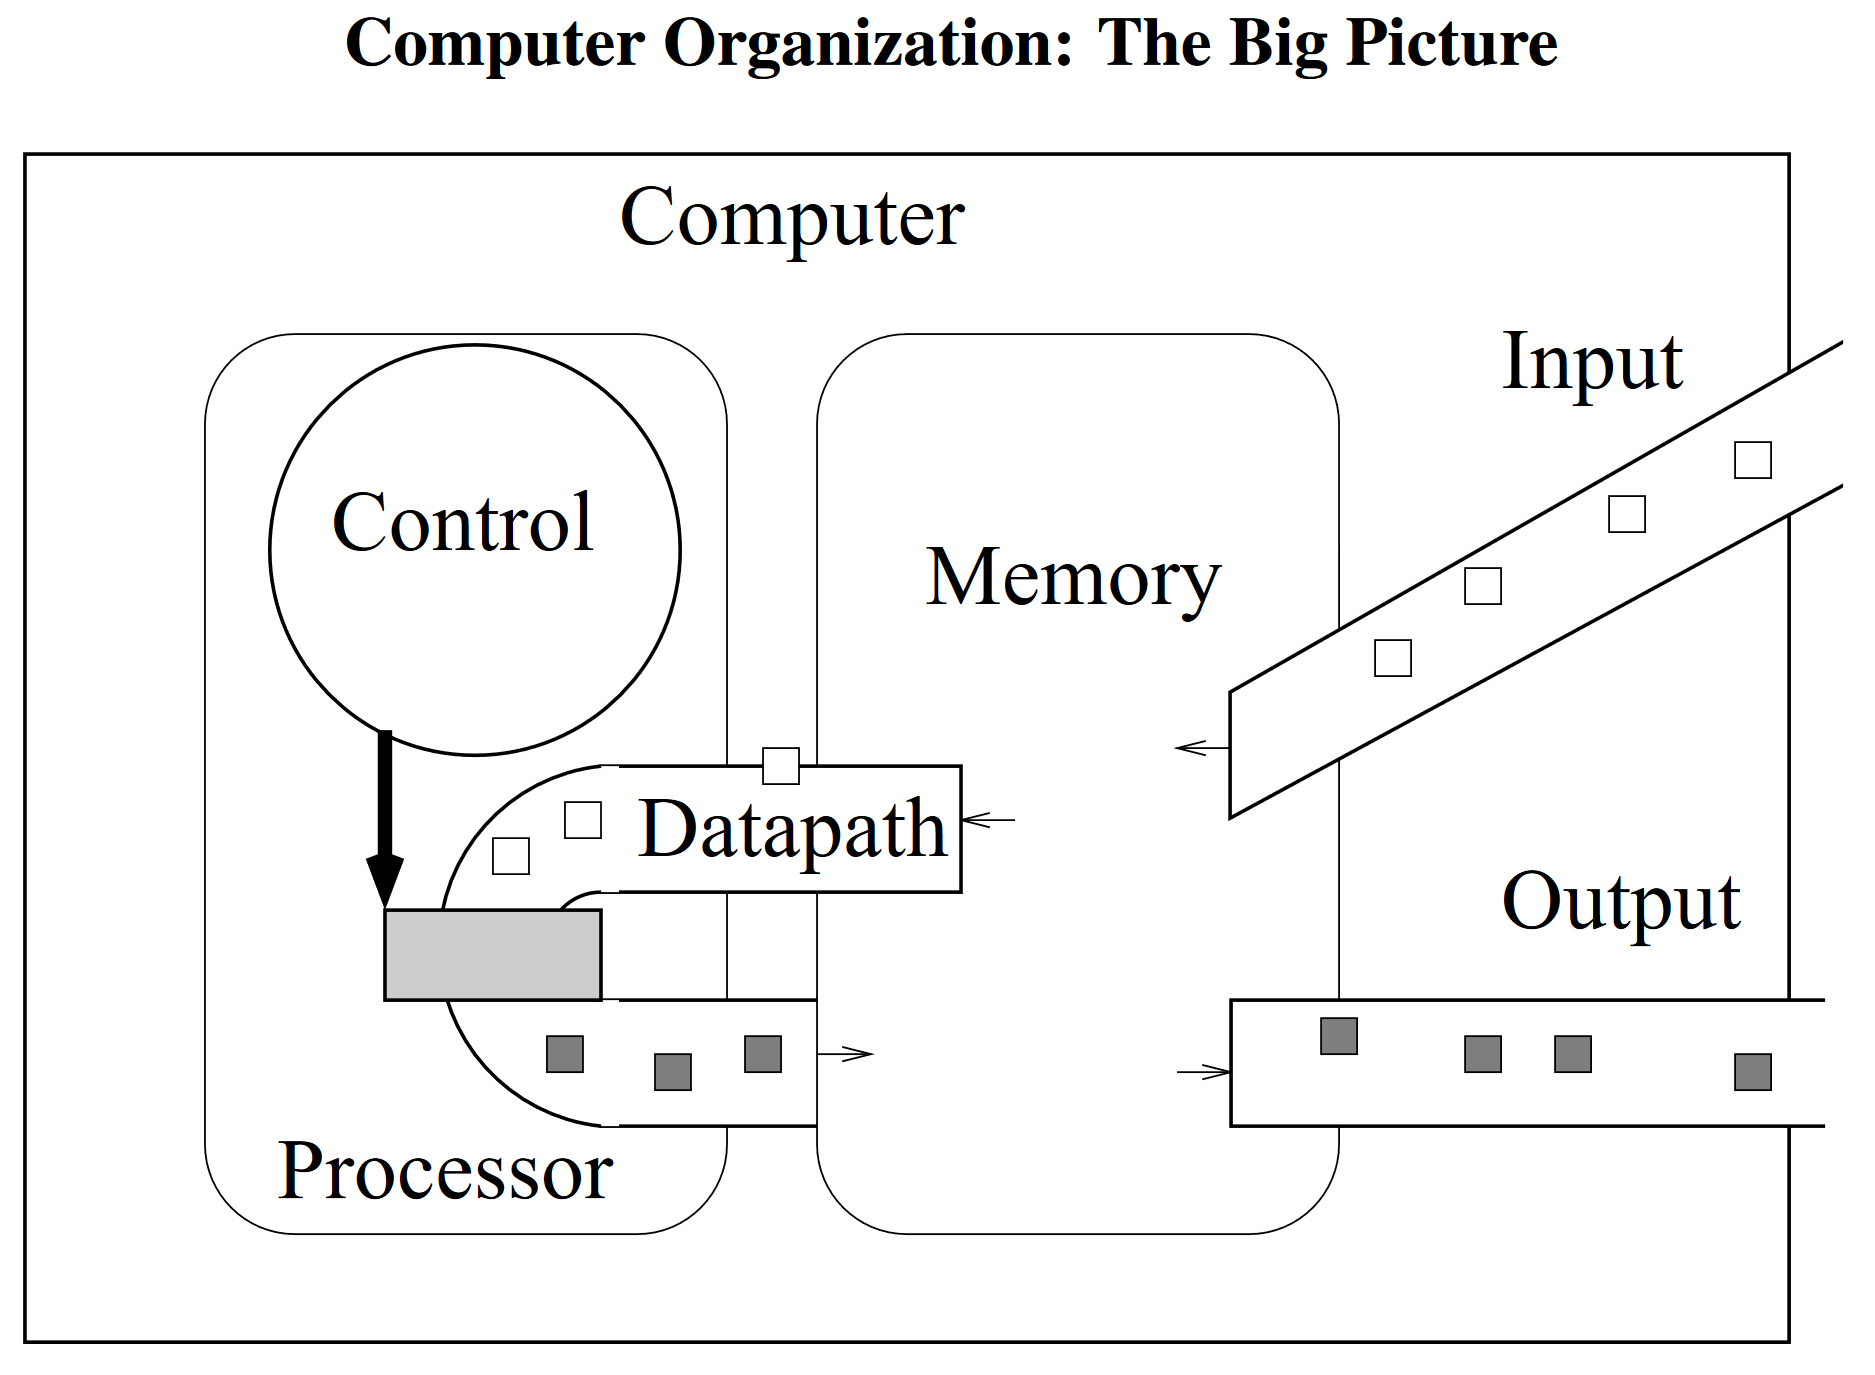
\includegraphics[width=0.75\textwidth]{figures/big-picture.png}
  \caption{The five classic components of a computer: control and datapath
  (together the processor), memory, input and output.}
\end{figure}

\begin{itemize}
  \item \textbf{Datapath}: the hardware that actually performs operations on
    data (registers, ALU, multiplexers, buses). Formally, the datapath is
    the collection of hardware units that come together to execute an
    instruction.
  \item \textbf{Control}: tells the datapath, memory and I/O what to do
    according to the current instruction.
  \item \textbf{Memory}: holds both programs (instructions) and data while
    they are in use (stored-program concept).
  \item \textbf{Input} and \textbf{Output}: devices that bring data in and
    send results out.
\end{itemize}

\section{Assembly Language and MIPS}

Assembly language is a human-readable form of machine code. Each line
corresponds (essentially) to one machine instruction. Different operations
have different names (mnemonics) and different \emph{formats}.

\begin{definition}
\textbf{MIPS} (originally ``Microprocessor without Interlocked Pipeline
Stages'') is a \textbf{RISC} (Reduced Instruction Set Computer) architecture:
\begin{enumerate}
  \item it provides only very basic operations, each doing a small amount of
    work;
  \item all instructions are the same size: in this course, a 32-bit word
    (64-bit versions of MIPS exist but we use the 32-bit one);
  \item the first six bits of every instruction are the \textbf{opcode}.
\end{enumerate}
\end{definition}

The execution of an instruction in hardware is divided into five steps:
instruction fetch, instruction decode/register read, execute (ALU), memory
access, and register write-back. This five-way split will reappear when we
pipeline the processor.

\subsection{Registers}

\begin{definition}
A \textbf{register} is a small, very fast storage location inside the
processor. It plays a role similar to a temporary variable in a high-level
language. MIPS has 32 general-purpose registers, each 32 bits wide.
\end{definition}

\begin{example}
Compile \lstinline[style=c]|f = (g + h) - (i + j);| where the variables
$f, g, h, i, j$ live in registers \code{\$s1}, \ldots, \code{\$s5}:

\begin{lstlisting}[style=mips]
add $t0, $s2, $s3    # t0 = g + h
add $t1, $s4, $s5    # t1 = i + j
sub $s1, $t0, $t1    # f  = t0 - t1
\end{lstlisting}
Since an instruction has only two source operands, we need temporaries
(\code{\$t0}, \code{\$t1}) to hold intermediate results.
\end{example}

Two issues already show up in this tiny example:
\begin{itemize}
  \item \textbf{Data dependency}: the \code{sub} needs the results of both
    \code{add}s, so it cannot run before them. This matters a lot once
    instructions overlap in a pipeline.
  \item \textbf{Overflow}: a 32-bit register cannot hold every sum; adding
    two large numbers may produce a result that does not fit.
\end{itemize}

\subsection{Instruction addresses}

Instructions are stored in memory one after the other. Since every MIPS
instruction is 4 bytes, consecutive instructions are at addresses
$0, 4, 8, 12, \ldots$:

\begin{center}
\begin{tabular}{rl}
\toprule
Address & Instruction \\
\midrule
0  & \code{add \$3, \$2, \$1} \\
4  & \code{sub \ldots} \\
8  & \code{sub \ldots} \\
12 & \code{sub \ldots} \\
\bottomrule
\end{tabular}
\end{center}

\subsection{The three MIPS instruction formats}

The \emph{format} of an instruction describes how many operands it has and
of what type.
\begin{itemize}
  \item \textbf{R-format} (register): \code{add \$1, \$2, \$3} adds the
    contents of \code{\$2} and \code{\$3} and stores the result in
    \code{\$1}. Often written \code{add rd, rs, rt} where \code{rd} is the
    destination register.
  \item \textbf{I-format} (immediate): \code{addi \$1, \$2, 100} adds the
    constant 100 to \code{\$2} and stores the result in \code{\$1}.
  \item \textbf{J-format} (jump): \code{j 28}, used for unconditional
    jumps (details later).
\end{itemize}

\subsection{Jumping counts words, not bytes}

When we say ``jump to instruction 40'' we mean the 40th instruction (word),
so the program counter moves to byte address $40 \times 4 = 160$. Because
every instruction is 4 bytes, the low two bits of an instruction address are
always $00$, and MIPS saves encoding space by storing word offsets and
multiplying by 4 in hardware.

\section*{Summary}
\begin{itemize}
  \item CS 251 is about how a processor is built: ISA, digital logic,
    datapath and control, pipelining, memory hierarchy.
  \item The ISA is the hardware/software contract; MIPS is a simple 32-bit
    RISC ISA with fixed-length instructions and a 6-bit opcode.
  \item A computer = datapath + control (processor) + memory + input + output.
  \item Registers are fast local storage; MIPS has 32 of them.
  \item Three formats: R (three registers), I (two registers + constant),
    J (jump target). Instruction addresses go up by 4.
\end{itemize}

\chapter{MIPS Basics: Five Instructions}

Before building any hardware, we need to know what the hardware is supposed
to do. For most of the course we use a tiny subset of MIPS consisting of five
instructions. They are enough to write real (if clumsy) programs and they
exercise every part of the datapath we will later build.

\section{The Machine Model}

\begin{itemize}
  \item 32 registers \code{\$0}--\code{\$31}, each holding a 32-bit
    \textbf{word}. Register \code{\$0} always reads as 0; writes to it are
    ignored.
  \item A \textbf{program counter} (PC) holding the address of the current
    instruction.
  \item A byte-addressed memory of $2^{32}$ bytes. Words are 4 bytes and
    word addresses must be multiples of 4 (\emph{alignment}).
  \item MIPS is a \textbf{load/store architecture}: arithmetic works only on
    registers; memory is touched only by loads and stores.
\end{itemize}

\section{The Five Instructions}

\begin{center}
\begin{tabular}{lll}
\toprule
Instruction & Meaning & Format \\
\midrule
\code{add \$d, \$s, \$t} & $\$d \gets \$s + \$t$ & R \\
\code{sub \$d, \$s, \$t} & $\$d \gets \$s - \$t$ & R \\
\code{lw \$t, i(\$s)} & $\$t \gets \mathrm{MEM}[\$s + i]$ & I \\
\code{sw \$t, i(\$s)} & $\mathrm{MEM}[\$s + i] \gets \$t$ & I \\
\code{beq \$s, \$t, i} & if $\$s = \$t$ then $PC \gets PC + 4 + 4i$ & I \\
\bottomrule
\end{tabular}
\end{center}

In every case, after the instruction (unless a branch is taken) the PC
advances by 4. Here $i$ is a 16-bit signed constant (immediate).

\subsection{Arithmetic: \code{add} and \code{sub}}

Both take three registers. The order of operands in assembly is destination
first. There is no ``move'' instruction; to copy a register use
\code{add \$d, \$s, \$0}.

\subsection{Memory: \code{lw} and \code{sw}}

The address is computed as \emph{base register + signed offset}. This
``displacement'' addressing mode is natural for arrays and structs:

\begin{example}
Suppose \code{\$1} holds the address of an array \code{A} of 32-bit integers.
Then \code{A[3]} is at byte offset $3 \times 4 = 12$:
\begin{lstlisting}[style=mips]
lw  $2, 12($1)     # $2 = A[3]
add $2, $2, $2     # double it
sw  $2, 12($1)     # A[3] = $2
\end{lstlisting}
\end{example}

\begin{figure}[H]
\centering
\begin{tikzpicture}[>=Stealth, thick, font=\small, x=1.6cm, y=1cm]
  \foreach \k in {0,...,5} {
    \pgfmathtruncatemacro{\off}{4*\k}
    \draw (\k,0) rectangle (\k+1,1);
    \node at (\k+0.5,0.5) {\code{A[\k]}};
    \node[font=\scriptsize, below] at (\k+0.5,0) {$+\off$};
    \foreach \b in {1,2,3} \draw[gray!50, thin] (\k+\b/4,0) -- (\k+\b/4,0.15);
  }
  \fill[blue!15] (3,0) rectangle (4,1); \draw (3,0) rectangle (4,1);
  \node at (3.5,0.5) {\code{A[3]}};
  \node[draw, rounded corners, above=1.0cm] (r1) at (0.5,1) {\code{\$1} = base address};
  \draw[->] (r1.south) -- (0.05,1);
  \draw[->, blue!60!black] (0.05,1.25) -- node[above, font=\scriptsize]{offset 12 bytes $= 3 \times 4$} (3.0,1.25);
  \node[font=\scriptsize, anchor=east] at (-0.05,-0.3) {byte offset};
\end{tikzpicture}
\caption{\code{lw \$2, 12(\$1)}: each word is 4 bytes (tick marks), so
\code{A[3]} starts 12 bytes after the base address in \code{\$1}.}
\end{figure}

\begin{important}[Pitfall: byte offsets]
Offsets are in \emph{bytes}, not elements. \code{A[k]} for word arrays is at
offset $4k$. Forgetting the factor of 4 is the most common beginner error.
\end{important}

\subsection{Branching: \code{beq}}

\code{beq} compares two registers. If equal, it jumps $i$ \emph{instructions}
relative to the instruction \emph{after} the branch (because the PC has
already been incremented by 4 when the branch is evaluated). So
\code{beq \$0, \$0, -1} is an infinite loop and \code{beq \$0, \$0, 0} does
nothing useful.

\section{Writing Programs with Five Instructions}

\begin{example}[If statement]
Compute \lstinline[style=c]|if (a == b) c = a + b; else c = a - b;| with
\code{a, b, c} in \code{\$1, \$2, \$3}.
\begin{lstlisting}[style=mips]
      beq $1, $2, 2      # if a == b skip the next two instructions
      sub $3, $1, $2     # else part
      beq $0, $0, 1      # unconditional "jump" over the then part
      add $3, $1, $2     # then part
                         # continue here
\end{lstlisting}
\code{beq \$0, \$0, k} is the standard trick for an unconditional branch,
since \code{\$0 = \$0} is always true.
\end{example}

\begin{example}[Loop: sum an array]
\code{\$1} = address of array, \code{\$2} = number of elements $n$,
\code{\$4} holds the constant 4 and \code{\$5} holds the constant 1 (assume
they were set up for us, since we have no immediate arithmetic yet).
Result in \code{\$3}.
\begin{lstlisting}[style=mips]
      add $3, $0, $0     # sum = 0
loop: beq $2, $0, 5      # if n == 0 exit (skip 5 instructions)
      lw  $6, 0($1)      # t = *p
      add $3, $3, $6     # sum += t
      add $1, $1, $4     # p += 4  (next word)
      sub $2, $2, $5     # n -= 1
      beq $0, $0, -6     # back to loop
                         # exit
\end{lstlisting}
Counting the branch offset: from the instruction after
\code{beq \$0,\$0,-6}, we must go back 6 instructions to reach \code{loop}.

\begin{figure}[H]
\centering
\begin{tikzpicture}[>=Stealth, thick, font=\small, y=0.55cm]
  \foreach \i/\txt in {0/{add \$3, \$0, \$0}, 1/{loop: beq \$2, \$0, 5}, 2/{lw \$6, 0(\$1)},
      3/{add \$3, \$3, \$6}, 4/{add \$1, \$1, \$4}, 5/{sub \$2, \$2, \$5},
      6/{beq \$0, \$0, -6}, 7/{exit: \ldots}} {
    \pgfmathtruncatemacro{\addr}{4*\i}
    \node[font=\scriptsize, anchor=east] at (-1.2,-\i) {\addr};
    \node[draw, anchor=west, minimum width=3.6cm, minimum height=0.5cm, font=\ttfamily\scriptsize] at (0,-\i) {\txt};
  }
  % forward branch: PC+4 = instruction 2, +5 instructions = 7
  \draw[->, blue!60!black] (3.7,-2) -- ++(0.6,0) |- node[pos=0.25, sloped, above, font=\scriptsize]{$+5$ from $PC+4$} (3.7,-7);
  \draw[blue!60!black, densely dotted] (3.7,-1) -- ++(0.25,0) |- (3.7,-2);
  % backward branch: PC+4 = instruction 7, -6 instructions = 1
  \draw[->, red!60!black] (0,-7) -- ++(-0.8,0) |- node[pos=0.25, sloped, above, font=\scriptsize]{$-6$ from $PC+4$} (0,-1);
  \draw[red!60!black, densely dotted] (0,-6) -- ++(-0.35,0) |- (0,-7);
  \node[font=\scriptsize] at (-1.45,0.9) {addr};
\end{tikzpicture}
\caption{Branch offsets are counted in instructions from $PC+4$ (dotted
step), not from the branch itself.}
\end{figure}
\end{example}

\section{Machine Encoding Preview}

Every instruction is 32 bits. The first 6 bits are the opcode.

\begin{center}
\begin{tabular}{l|c|c|c|c|c|c|}
\cline{2-7}
R & op (6) & rs (5) & rt (5) & rd (5) & shamt (5) & funct (6) \\
\cline{2-7}
I & op (6) & rs (5) & rt (5) & \multicolumn{3}{c|}{immediate (16)} \\
\cline{2-7}
\end{tabular}
\end{center}

\begin{center}
\begin{tabular}{lcc}
\toprule
Instruction & opcode & funct \\
\midrule
\code{add} & 000000 & 100000 (0x20) \\
\code{sub} & 000000 & 100010 (0x22) \\
\code{lw}  & 100011 (0x23) & -- \\
\code{sw}  & 101011 (0x2B) & -- \\
\code{beq} & 000100 (0x04) & -- \\
\bottomrule
\end{tabular}
\end{center}

\begin{example}
Encode \code{add \$3, \$1, \$2}: op = 0, rs = 1, rt = 2, rd = 3,
shamt = 0, funct = 0x20.
\[
\underbrace{000000}_{op}\,\underbrace{00001}_{rs}\,\underbrace{00010}_{rt}\,
\underbrace{00011}_{rd}\,\underbrace{00000}_{shamt}\,\underbrace{100000}_{funct}
= \texttt{0x00221820}.
\]

\begin{center}
\begin{tikzpicture}[font=\small, x=0.36cm, y=0.9cm]
  \foreach \a/\b/\name/\val in {0/6/op/000000, 6/11/rs/00001, 11/16/rt/00010,
      16/21/rd/00011, 21/26/shamt/00000, 26/32/funct/100000} {
    \draw[thick] (\a,0) rectangle (\b,1);
    \node[font=\ttfamily\scriptsize] at ({(\a+\b)/2},0.5) {\val};
    \node[font=\scriptsize, above] at ({(\a+\b)/2},1) {\name};
  }
  \foreach \x/\v in {3/0, 8.5/1, 13.5/2, 18.5/3, 23.5/0, 29/{0x20}}
    \node[font=\scriptsize, gray!70!black] at (\x,-0.3) {\v};
  \node[font=\scriptsize, anchor=east] at (-0.2,0.5) {bit 31};
  \node[font=\scriptsize, anchor=west] at (32.2,0.5) {bit 0};
\end{tikzpicture}
\end{center}
Note that in assembly the destination comes first, but in the encoding
\code{rd} comes third.
\end{example}

\begin{example}
Encode \code{lw \$5, -8(\$29)}: op = 0x23, rs = 29, rt = 5, imm = $-8$
= \code{0xFFF8}. Bits: \code{100011 11101 00101 1111111111111000}
= \code{0x8FA5FFF8}.
\end{example}

\section*{Summary}
\begin{itemize}
  \item Five instructions: \code{add}, \code{sub}, \code{lw}, \code{sw},
    \code{beq}. Two R-format, three I-format.
  \item Memory addresses are base + signed byte offset; words are aligned.
  \item Branch offsets count instructions relative to $PC+4$.
  \item \code{beq \$0, \$0, k} acts as an unconditional branch.
  \item These five instructions drive the design of the single-cycle
    datapath later in the course.
\end{itemize}

\chapter{Digital Logic: Combinational Circuits}

A processor is built out of transistors acting as switches. We abstract
transistors into \emph{logic gates}, gates into \emph{combinational
circuits} (whose outputs depend only on current inputs), and later add
memory to get \emph{sequential circuits}.

\section{Boolean Algebra}

Signals take one of two values, 0 (false, low voltage) and 1 (true, high
voltage). The basic operations are
\begin{itemize}
  \item AND: $A \cdot B$ (or $AB$), 1 iff both are 1;
  \item OR: $A + B$, 1 iff at least one is 1;
  \item NOT: $\overline{A}$ (or $A'$), flips the bit.
\end{itemize}
Derived operations: NAND $\overline{AB}$, NOR $\overline{A+B}$,
XOR $A \oplus B = A\overline{B} + \overline{A}B$, XNOR $\overline{A\oplus B}$.

\begin{center}
\begin{tabular}{cc|cccccc}
\toprule
$A$ & $B$ & AND & OR & NAND & NOR & XOR & XNOR \\
\midrule
0 & 0 & 0 & 0 & 1 & 1 & 0 & 1 \\
0 & 1 & 0 & 1 & 1 & 0 & 1 & 0 \\
1 & 0 & 0 & 1 & 1 & 0 & 1 & 0 \\
1 & 1 & 1 & 1 & 0 & 0 & 0 & 1 \\
\bottomrule
\end{tabular}
\end{center}

\subsection{Laws}

\begin{center}
\begin{tabular}{lll}
\toprule
Law & AND form & OR form \\
\midrule
Identity & $A\cdot 1 = A$ & $A + 0 = A$ \\
Null & $A \cdot 0 = 0$ & $A + 1 = 1$ \\
Idempotent & $AA = A$ & $A + A = A$ \\
Complement & $A\overline{A} = 0$ & $A + \overline{A} = 1$ \\
Commutative & $AB = BA$ & $A+B = B+A$ \\
Associative & $(AB)C = A(BC)$ & $(A+B)+C = A+(B+C)$ \\
Distributive & $A(B+C) = AB+AC$ & $A + BC = (A+B)(A+C)$ \\
Absorption & $A(A+B) = A$ & $A + AB = A$ \\
De Morgan & $\overline{AB} = \overline{A}+\overline{B}$ &
  $\overline{A+B} = \overline{A}\,\overline{B}$ \\
\bottomrule
\end{tabular}
\end{center}

Note the second distributive law $A + BC = (A+B)(A+C)$, which has no
analogue in ordinary arithmetic. Every law has a \emph{dual} obtained by
swapping AND/OR and 0/1.

\begin{example}
Simplify $F = \overline{A}B + AB + A\overline{B}$.
\[
F = (\overline{A}+A)B + A\overline{B} = B + A\overline{B}
  = (B + A)(B + \overline{B}) = A + B.
\]
\end{example}

\section{Gates}

\begin{figure}[H]
\centering
\begin{tikzpicture}[circuit logic US, every circuit symbol/.style={thick}]
  \node[and gate, inputs=nn] (a) at (0,0) {};
  \node[or gate, inputs=nn] (o) at (2.5,0) {};
  \node[not gate] (n) at (5,0) {};
  \node[nand gate, inputs=nn] (na) at (7,0) {};
  \node[xor gate, inputs=nn] (x) at (9.5,0) {};
  \node[below=4mm] at (a) {AND};
  \node[below=4mm] at (o) {OR};
  \node[below=4mm] at (n) {NOT};
  \node[below=4mm] at (na) {NAND};
  \node[below=4mm] at (x) {XOR};
\end{tikzpicture}
\caption{Standard (US) gate symbols. A bubble on an output means inversion.}
\end{figure}

\begin{important}[Universality]
NAND alone is \emph{functionally complete}: $\overline{A} = \overline{AA}$,
$AB = \overline{\overline{AB}}$, $A+B = \overline{\overline{A}\,\overline{B}}$.
The same is true for NOR. Real CMOS hardware prefers NAND/NOR because they
need fewer transistors than AND/OR.
\end{important}

\section{Truth Tables and Canonical Forms}

Any Boolean function of $n$ inputs is described by a truth table with $2^n$
rows.

\begin{definition}
A \textbf{minterm} is a product (AND) containing every variable once, either
plain or complemented; it is 1 in exactly one row. The \textbf{sum of
products (SOP)} form is the OR of the minterms for rows where $F = 1$.
Dually, a \textbf{maxterm} is a sum that is 0 in exactly one row, and the
\textbf{product of sums (POS)} form ANDs the maxterms of the rows where
$F = 0$.
\end{definition}

\begin{example}[Majority function]
$F(A,B,C) = 1$ iff at least two inputs are 1.
\begin{center}
\begin{tabular}{ccc|c}
\toprule
$A$ & $B$ & $C$ & $F$ \\
\midrule
0&0&0&0\\ 0&0&1&0\\ 0&1&0&0\\ 0&1&1&1\\
1&0&0&0\\ 1&0&1&1\\ 1&1&0&1\\ 1&1&1&1\\
\bottomrule
\end{tabular}
\end{center}
SOP: $F = \overline{A}BC + A\overline{B}C + AB\overline{C} + ABC
= \sum m(3,5,6,7)$. This simplifies to $F = AB + AC + BC$.
\end{example}

\section{Karnaugh Maps}

A K-map arranges the truth table in a grid whose rows and columns follow
\textbf{Gray code} order (00, 01, 11, 10) so that physically adjacent cells
differ in exactly one variable. Adjacent 1s can then be combined, since
$XY + X\overline{Y} = X$.

\textbf{Rules for grouping}:
\begin{enumerate}
  \item Groups must be rectangles of size $1, 2, 4, 8, \ldots$ (powers of 2).
  \item Groups may wrap around the edges (the map is a torus).
  \item Make groups as large as possible, and use as few as possible; every
    1 must be covered; overlapping is allowed.
  \item Don't-care entries (X) may be included in a group if that helps,
    but need not be covered.
\end{enumerate}
Each group of $2^k$ cells eliminates $k$ variables.

\begin{example}
Majority function K-map (rows $A$, columns $BC$):
\begin{center}
\begin{tabular}{c|cccc}
$A \backslash BC$ & 00 & 01 & 11 & 10 \\
\hline
0 & 0 & 0 & 1 & 0 \\
1 & 0 & 1 & 1 & 1 \\
\end{tabular}
\end{center}
Three groups of two: the column $BC = 11$ gives $BC$; cells $(1,01),(1,11)$
give $AC$; cells $(1,11),(1,10)$ give $AB$. So $F = AB + AC + BC$.

\begin{center}
\begin{tikzpicture}[x=1cm, y=0.8cm, font=\small]
  \foreach \c/\lab in {0/00, 1/01, 2/11, 3/10} \node at (\c+0.5,0.35) {\lab};
  \foreach \r in {0,1} \node at (-0.35,-\r-0.5) {\r};
  \node at (-0.45,0.35) {\scriptsize $A\backslash BC$};
  \foreach \c in {0,...,4} \draw (\c,0) -- (\c,-2);
  \foreach \r in {0,1,2} \draw (0,-\r) -- (4,-\r);
  \foreach \r/\row in {0/{0,0,1,0}, 1/{0,1,1,1}} {
    \foreach \v [count=\c from 0] in \row \node at (\c+0.5,-\r-0.5) {\v};
  }
  \draw[very thick, red!70!black, rounded corners] (2.12,-0.1) rectangle (2.88,-1.9);
  \draw[very thick, blue!70!black, rounded corners] (1.05,-1.15) rectangle (2.95,-1.85);
  \draw[very thick, green!50!black, rounded corners, dashed] (2.05,-1.08) rectangle (3.92,-1.92);
  \node[red!70!black, font=\scriptsize, right] at (4.2,-0.4) {$BC$};
  \node[blue!70!black, font=\scriptsize, right] at (4.2,-1.0) {$AC$};
  \node[green!50!black, font=\scriptsize, right] at (4.2,-1.6) {$AB$};
\end{tikzpicture}
\end{center}
The three overlapping groups of the majority K-map; overlapping is allowed
because $X + X = X$.
\end{example}

\begin{example}[Four variables]
$F(A,B,C,D) = \sum m(0,2,5,7,8,10,13,15)$.
\begin{center}
\begin{tabular}{c|cccc}
$AB \backslash CD$ & 00 & 01 & 11 & 10 \\
\hline
00 & 1 & 0 & 0 & 1 \\
01 & 0 & 1 & 1 & 0 \\
11 & 0 & 1 & 1 & 0 \\
10 & 1 & 0 & 0 & 1 \\
\end{tabular}
\end{center}
The four corners form one group (wrap-around) giving $\overline{B}\,\overline{D}$;
the middle $2\times 2$ block gives $BD$. Hence
$F = \overline{B}\,\overline{D} + BD = \overline{B \oplus D}$.

\begin{center}
\begin{tikzpicture}[x=1cm, y=0.8cm, font=\small]
  \foreach \c/\lab in {0/00, 1/01, 2/11, 3/10} \node at (\c+0.5,0.35) {\lab};
  \foreach \r/\lab in {0/00, 1/01, 2/11, 3/10} \node at (-0.35,-\r-0.5) {\lab};
  \node at (-0.55,0.35) {\scriptsize $AB\backslash CD$};
  \foreach \r/\row in {0/{1,0,0,1}, 1/{0,1,1,0}, 2/{0,1,1,0}, 3/{1,0,0,1}} {
    \foreach \v [count=\c from 0] in \row \node at (\c+0.5,-\r-0.5) {\v};
  }
  \foreach \c in {0,...,4} \draw (\c,0) -- (\c,-4);
  \foreach \r in {0,...,4} \draw (0,-\r) -- (4,-\r);
  \begin{scope}
    \clip (0,0) rectangle (4,-4);
    \foreach \x/\y in {0/0, 4/0, 0/-4, 4/-4}
      \draw[very thick, red!70!black, rounded corners] (\x-0.88,\y+0.88) rectangle (\x+0.88,\y-0.88);
  \end{scope}
  \draw[very thick, blue!70!black, rounded corners] (1.12,-1.12) rectangle (2.88,-2.88);
  \node[red!70!black, font=\scriptsize, right] at (4.2,-0.5) {corners: $\overline{B}\,\overline{D}$};
  \node[blue!70!black, font=\scriptsize, right] at (4.2,-2) {centre: $BD$};
\end{tikzpicture}
\end{center}
The red group wraps around both edges: the map is really a torus, so the
four corners are mutually adjacent.
\end{example}

\section{Combinational Building Blocks}

\subsection{Multiplexer}

A \textbf{multiplexer (mux)} selects one of several inputs using select
lines. A 2-to-1 mux with inputs $I_0, I_1$ and select $S$:
\[ Y = \overline{S} I_0 + S I_1. \]
A $2^k$-to-1 mux needs $k$ select bits. Muxes are everywhere in the
datapath: whenever a value may come from two places, a mux chooses.

\begin{figure}[H]
\centering
\begin{tikzpicture}[thick]
  \draw (0,0) -- (0,2) -- (1,1.6) -- (1,0.4) -- cycle;
  \draw (-0.8,1.5) node[left]{$I_0$} -- (0,1.5);
  \draw (-0.8,0.5) node[left]{$I_1$} -- (0,0.5);
  \draw (1,1) -- (1.8,1) node[right]{$Y$};
  \draw (0.5,0.2) -- (0.5,-0.5) node[below]{$S$};
  \node at (0.35,1.5) {\scriptsize 0};
  \node at (0.35,0.5) {\scriptsize 1};
\end{tikzpicture}
\caption{2-to-1 multiplexer.}
\end{figure}

A mux of $n$-bit buses is just $n$ one-bit muxes sharing the select line.

\subsection{Decoder}

An $n$-to-$2^n$ \textbf{decoder} has $n$ inputs and $2^n$ outputs; exactly
the output whose index equals the input value is 1. A 2-to-4 decoder:
$Y_0 = \overline{A_1}\,\overline{A_0}$, $Y_1 = \overline{A_1}A_0$,
$Y_2 = A_1\overline{A_0}$, $Y_3 = A_1A_0$. Decoders select a register
in the register file and a row in memory. An \textbf{encoder} does the
reverse.

\subsection{Adders}

\begin{definition}
A \textbf{half adder} adds two bits: $S = A \oplus B$, $C_{out} = AB$.
A \textbf{full adder} also takes a carry-in:
\[
S = A \oplus B \oplus C_{in}, \qquad
C_{out} = AB + AC_{in} + BC_{in}.
\]
\end{definition}

\begin{center}
\begin{tabular}{ccc|cc}
\toprule
$A$ & $B$ & $C_{in}$ & $C_{out}$ & $S$ \\
\midrule
0&0&0&0&0\\ 0&0&1&0&1\\ 0&1&0&0&1\\ 0&1&1&1&0\\
1&0&0&0&1\\ 1&0&1&1&0\\ 1&1&0&1&0\\ 1&1&1&1&1\\
\bottomrule
\end{tabular}
\end{center}

Notice $C_{out}$ is exactly the majority function.

\begin{figure}[H]
\centering
\begin{tikzpicture}[circuit logic US, huge circuit symbols, every circuit symbol/.style={thick}, thick]
  \node[xor gate, inputs=nn] (x1) at (2,1.2) {};
  \node[xor gate, inputs=nn] (x2) at (5.4,0.85) {};
  \node[and gate, inputs=nn] (a1) at (5.4,-0.6) {};
  \node[and gate, inputs=nn] (a2) at (5.4,-2) {};
  \node[or gate, inputs=nn] (o1) at (7.5,-1.3) {};
  % inputs
  \draw (-0.6,2.0) node[left]{$A$} -- (1.0,2.0) |- (x1.input 1);
  \draw (-0.6,0 |- x1.input 2) node[left]{$B$} -- (x1.input 2);
  \fill (0.0,2.0) circle (1.5pt);
  \draw (0.0,2.0) |- (a2.input 1);
  \fill (0.4,0 |- x1.input 2) circle (1.5pt);
  \draw (0.4,0 |- x1.input 2) |- (a2.input 2);
  \path (x2.input 2) ++(-0.4,0) coordinate (cu);
  \path (x2.input 2) ++(-0.9,0) coordinate (cb);
  \draw (-0.6,0.2) node[left]{$C_{in}$} -- (cu |- 0,0.2) -- (cu) -- (x2.input 2);
  \fill (cb |- 0,0.2) circle (1.5pt);
  \draw (cb |- 0,0.2) |- (a1.input 1);
  % A xor B to second xor and to the lower AND input
  \draw (x1.output) -- ++(0.5,0) coordinate(j) |- (x2.input 1);
  \draw (j) |- (a1.input 2);
  \fill (j) circle (1.5pt);
  % outputs
  \draw (x2.output) -- ++(2.4,0) node[right]{$S$};
  \draw (a1.output) -- ++(0.4,0) |- (o1.input 1);
  \draw (a2.output) -- ++(0.4,0) |- (o1.input 2);
  \draw (o1.output) -- ++(0.6,0) node[right]{$C_{out}$};
\end{tikzpicture}
\caption{A full adder from two half adders: $S = (A\oplus B)\oplus C_{in}$
and $C_{out} = AB + C_{in}(A\oplus B)$, which equals the majority function.}
\end{figure}

\paragraph{Ripple-carry adder.} Chain $n$ full adders, the carry-out of bit
$i$ feeding the carry-in of bit $i+1$. Simple, but the delay is $\Theta(n)$
because the carry may have to ripple through every stage.

\begin{figure}[H]
\centering
\begin{tikzpicture}[thick, box/.style={draw, minimum width=1.2cm, minimum height=1cm}]
  \foreach \i/\x in {3/0,2/2,1/4,0/6} {
    \node[box] (fa\i) at (\x,0) {FA};
    \draw (\x-0.25,1.2) node[above]{\scriptsize $A_\i$} -- (\x-0.25,0.5);
    \draw (\x+0.25,1.2) node[above]{\scriptsize $B_\i$} -- (\x+0.25,0.5);
    \draw (\x,-0.5) -- (\x,-1.1) node[below]{\scriptsize $S_\i$};
  }
  \draw[->] (fa0.west) -- (fa1.east);
  \draw[->] (fa1.west) -- (fa2.east);
  \draw[->] (fa2.west) -- (fa3.east);
  \draw[<-] (fa0.east) -- ++(0.7,0) node[right]{\scriptsize $C_0$};
  \draw[->] (fa3.west) -- ++(-0.7,0) node[left]{\scriptsize $C_4$};
\end{tikzpicture}
\caption{4-bit ripple-carry adder.}
\end{figure}

\paragraph{Carry-lookahead (idea).} Define \emph{generate} $g_i = A_iB_i$
and \emph{propagate} $p_i = A_i + B_i$. Then $c_{i+1} = g_i + p_ic_i$, which
can be expanded, e.g.\ $c_2 = g_1 + p_1g_0 + p_1p_0c_0$, so all carries are
computed in parallel in a constant number of gate levels (at the cost of
more gates). Hierarchical lookahead gives $\Theta(\log n)$ delay.

\paragraph{Subtraction.} $A - B = A + \overline{B} + 1$ in two's complement:
invert $B$ with XOR gates and set $C_0 = 1$. A single control bit
(\code{Binvert}) turns an adder into an adder/subtractor.

\subsection{The ALU}

The \textbf{arithmetic logic unit} computes one of several operations on two
32-bit inputs, chosen by a control input. A 1-bit ALU slice contains an AND
gate, an OR gate and a full adder, with a mux choosing the result;
32 slices are chained through the carries.

\begin{figure}[H]
\centering
\begin{tikzpicture}[circuit logic US, large circuit symbols, every circuit symbol/.style={thick}, thick, >=Stealth, font=\small]
  % gates
  \node[and gate, inputs=nn] (and) at (4,1.6) {};
  \node[or gate, inputs=nn] (or) at (4,0.4) {};
  \node[draw, minimum width=0.9cm, minimum height=1.1cm] (fa) at (4,-1.6) {$+$};
  % Binvert mux
  \draw (1.4,-0.6) -- (1.4,-2) -- (1.9,-1.8) -- (1.9,-0.8) -- cycle;
  \node[font=\tiny] at (1.55,-0.95) {0}; \node[font=\tiny] at (1.55,-1.65) {1};
  \node[not gate] (inv) at (0.55,-1.65) {};
  \draw (-0.6,-0.95) node[left]{$b$} -- (1.4,-0.95);
  \fill (-0.2,-0.95) circle (1.5pt);
  \draw (-0.2,-0.95) |- (inv.input);
  \draw (inv.output) -- (1.4,-1.65);
  \draw (1.65,-1.9) -- (1.65,-2.6) node[below, font=\scriptsize]{Binvert};
  % a bus
  \draw (-0.6,2.2) node[left]{$a$} -- (2.4,2.2) -- (2.4,-1.35);
  \foreach \y in {1.6,0.4} \fill (2.4,\y+0.2) circle (0pt);
  \draw (2.4,0 |- and.input 1) -- (and.input 1);
  \draw (2.4,0 |- or.input 1) -- (or.input 1);
  \draw (2.4,-1.35) -- ($(fa.west)+(0,0.25)$);
  \fill (2.4,0 |- and.input 1) circle (1.5pt);
  \fill (2.4,0 |- or.input 1) circle (1.5pt);
  % b bus
  \draw (1.9,-1.3) -- (2.9,-1.3);
  \draw (2.9,-1.85) -- (2.9,0 |- and.input 2) -- (and.input 2);
  \draw (2.9,0 |- or.input 2) -- (or.input 2);
  \draw (2.9,-1.85) -- ($(fa.west)+(0,-0.25)$);
  \fill (2.9,-1.3) circle (1.5pt);
  \fill (2.9,0 |- or.input 2) circle (1.5pt);
  % operation mux
  \draw (5.6,2.3) -- (5.6,-2.3) -- (6.2,-1.7) -- (6.2,1.7) -- cycle;
  \node[font=\tiny] at (5.75,1.6) {0}; \node[font=\tiny] at (5.75,0.4) {1};
  \node[font=\tiny] at (5.75,-1.6) {2};
  \draw (and.output) -- (5.6,1.6);
  \draw (or.output) -- (5.6,0.4);
  \draw (fa.east) -- (5.6,-1.6);
  \draw (6.2,0) -- (6.8,0) node[right]{Result};
  \draw (5.9,2) -- (5.9,2.7) node[above, font=\scriptsize]{Operation};
  % carries
  \draw[<-] (fa.north) -- ++(0,0.5) node[above, font=\scriptsize]{CarryIn};
  \draw[->] (fa.south) -- ++(0,-0.6) node[below, font=\scriptsize]{CarryOut};
\end{tikzpicture}
\caption{One 1-bit ALU slice: AND, OR and a full adder compute in
parallel and the \code{Operation} mux picks one. \code{Binvert} selects
$\overline{b}$ for subtraction.}
\end{figure}

\begin{center}
\begin{tabular}{cl}
\toprule
ALU control & Function \\
\midrule
0000 & AND \\
0001 & OR \\
0010 & add \\
0110 & subtract \\
0111 & set on less than \\
1100 & NOR \\
\bottomrule
\end{tabular}
\end{center}
The 4-bit control is \code{Ainvert}, \code{Bnegate} (= \code{Binvert} and
$C_0$), and a 2-bit operation select. Extra outputs:
\begin{itemize}
  \item \textbf{Zero}: 1 if the result is 0 (NOR of all result bits); used
    by \code{beq} (subtract and test Zero).
  \item \textbf{Overflow}: for signed add, $C_{n} \oplus C_{n-1}$ (carry into
    the sign bit differs from carry out).
  \item \textbf{Set on less than}: compute $A - B$; the sign bit of the
    result (corrected for overflow) is routed to bit 0 of the output, all
    other bits 0.
\end{itemize}

\begin{figure}[H]
\centering
\begin{tikzpicture}[thick]
  \draw (0,0) -- (0,1.2) -- (0.4,1.6) -- (0,2) -- (0,3.2) -- (1.6,2.4) -- (1.6,0.8) -- cycle;
  \node at (0.9,1.6) {ALU};
  \draw (-1,2.6) node[left]{$A$} -- (0,2.6);
  \draw (-1,0.6) node[left]{$B$} -- (0,0.6);
  \draw (1.6,1.8) -- (2.6,1.8) node[right]{Result};
  \draw (1.6,1.2) -- (2.6,1.2) node[right]{Zero};
  \draw (0.8,-0.5) node[below]{ALU control} -- (0.8,0.4);
\end{tikzpicture}
\caption{ALU symbol.}
\end{figure}

\section{Timing}

Gates have \emph{propagation delay}. The delay of a combinational circuit is
the delay along its \textbf{critical path} (longest path from any input to
any output). This will determine the clock period of the processor.

\section*{Summary}
\begin{itemize}
  \item Boolean algebra laws (especially De Morgan) let us manipulate
    expressions; NAND and NOR are universal.
  \item Truth table $\to$ SOP via minterms $\to$ simplify with K-maps
    (Gray code, power-of-two groups, wrap-around, don't cares).
  \item Building blocks: mux (select), decoder (one-hot), full adder,
    ripple-carry and carry-lookahead adders, ALU with Zero and Overflow.
  \item Subtraction = add the complement plus 1.
\end{itemize}

\chapter{Digital Logic: Sequential Circuits}

Combinational circuits have no memory: outputs are a function of current
inputs only. To build registers, the PC and memory, we need circuits whose
outputs also depend on their \emph{state}. These are \textbf{sequential
circuits}. The key ingredient is feedback.

\section{Latches}

\subsection{SR latch}

Two cross-coupled NOR gates form an \textbf{SR (set--reset) latch}.

\begin{figure}[H]
\centering
\begin{tikzpicture}[circuit logic US, every circuit symbol/.style={thick}, thick]
  \node[nor gate, inputs=nn] (n1) at (0,1.2) {};
  \node[nor gate, inputs=nn] (n2) at (0,-1.2) {};
  \draw (n1.input 1) -- ++(-1,0) node[left]{$R$};
  \draw (n2.input 2) -- ++(-1,0) node[left]{$S$};
  \draw (n1.output) -- ++(1.2,0) node[right]{$Q$};
  \draw (n2.output) -- ++(1.2,0) node[right]{$\overline{Q}$};
  \draw (n1.output) ++(0.5,0) -- ++(0,-0.8) -- ($(n2.input 1)+(-0.4,0.4)$) -- ++(0,-0.4) -- (n2.input 1);
  \draw (n2.output) ++(0.5,0) -- ++(0,0.8) -- ($(n1.input 2)+(-0.4,-0.4)$) -- ++(0,0.4) -- (n1.input 2);
\end{tikzpicture}
\caption{SR latch from two NOR gates.}
\end{figure}

\begin{center}
\begin{tabular}{cc|cl}
\toprule
$S$ & $R$ & $Q_{next}$ & \\
\midrule
0 & 0 & $Q$ & hold (remember) \\
0 & 1 & 0 & reset \\
1 & 0 & 1 & set \\
1 & 1 & -- & forbidden ($Q = \overline{Q} = 0$, unpredictable after) \\
\bottomrule
\end{tabular}
\end{center}

\subsection{D latch}

To avoid the forbidden state, a \textbf{D latch} derives $S = D\cdot C$ and
$R = \overline{D}\cdot C$ from a data input $D$ and an enable/clock $C$.
When $C = 1$ the latch is \emph{transparent} ($Q$ follows $D$); when $C = 0$
it holds its value.

\section{Clocks and Flip-Flops}

A \textbf{clock} is a periodic signal. Its \emph{period} is the time of one
cycle; the frequency is the reciprocal (a 1\,ns period means 1\,GHz). In
\textbf{edge-triggered} design, state changes only at a clock edge (we use
the rising edge), so all state elements update simultaneously and
combinational logic has a whole cycle to settle in between.

\begin{definition}
A \textbf{D flip-flop} samples $D$ at the rising clock edge and holds that
value in $Q$ until the next rising edge. It can be built from two D latches
in a \emph{master--slave} arrangement: the master is transparent while
$C = 0$, the slave while $C = 1$, so the value passes through only at the
$0 \to 1$ transition.
\end{definition}

\begin{important}[Latch vs flip-flop]
A latch is \emph{level}-sensitive (transparent for the whole time the clock
is high). A flip-flop is \emph{edge}-triggered. Using latches in a loop with
combinational logic can cause a value to race around the loop several times
in one cycle; flip-flops prevent this.
\end{important}

\begin{figure}[H]
\centering
\begin{tikzpicture}[x=1.6cm, y=0.8cm, font=\small]
  \fill[blue!8] (1,-0.2) rectangle (2,4.0);
  \fill[blue!8] (3,-0.2) rectangle (4,4.0);
  \fill[blue!8] (5,-0.2) rectangle (6,4.0);
  \foreach \x in {1,3,5} \draw[red!60!black, densely dashed] (\x,-0.2) -- (\x,4.0);
  \node[anchor=east] at (-0.1,3.3) {$C$ (clock)};
  \node[anchor=east] at (-0.1,2.3) {$D$};
  \node[anchor=east] at (-0.1,1.3) {$Q$, D latch};
  \node[anchor=east] at (-0.1,0.3) {$Q$, flip-flop};
  \draw[thick] (0,3) -- (1,3) -- (1,3.6) -- (2,3.6) -- (2,3) -- (3,3) -- (3,3.6) -- (4,3.6) -- (4,3) -- (5,3) -- (5,3.6) -- (6,3.6);
  \draw[thick] (0,2) -- (0.5,2) -- (0.5,2.6) -- (1.4,2.6) -- (1.4,2) -- (1.7,2) -- (1.7,2.6) -- (2.6,2.6) -- (2.6,2) -- (3.5,2) -- (3.5,2.6) -- (4.3,2.6) -- (4.3,2) -- (6,2);
  \draw[thick] (0,1) -- (1,1) -- (1,1.6) -- (1.4,1.6) -- (1.4,1) -- (1.7,1) -- (1.7,1.6) -- (3,1.6) -- (3,1) -- (3.5,1) -- (3.5,1.6) -- (5,1.6) -- (5,1) -- (6,1);
  \draw[thick] (0,0) -- (1,0) -- (1,0.6) -- (3,0.6) -- (3,0) -- (6,0);
  \node[font=\scriptsize, blue!50!black] at (1.5,4.25) {transparent};
  \node[font=\scriptsize, red!60!black] at (3,4.25) {rising edge};
\end{tikzpicture}
\caption{A D latch (level-sensitive) passes every change of $D$ while the
clock is high (shaded); a D flip-flop only samples $D$ at the rising edges
(dashed), so it ignores the short pulse in $D$ during the first high phase.}
\end{figure}

\paragraph{Timing constraints.} The input must be stable for a
\emph{setup time} before the edge and a \emph{hold time} after it; the output
changes a \emph{clock-to-Q} delay after the edge. Therefore
\[
T_{clock} \ge t_{clk\to Q} + t_{\text{critical path}} + t_{setup}.
\]

\begin{figure}[H]
\centering
\begin{tikzpicture}[x=1cm, y=0.8cm, font=\small, >=Stealth]
  % clock
  \draw[thick] (0,2) -- (1,2) -- (1,2.6) -- (5,2.6) -- (5,2) -- (9,2) -- (9,2.6) -- (10.5,2.6);
  \node[anchor=east] at (-0.1,2.3) {clock};
  % register output Q and combinational logic output
  \draw[thick] (0,1) -- (1.6,1) (0,1.6) -- (1.6,1.6);
  \draw[thick] (1.6,1) -- (1.8,1.6) (1.6,1.6) -- (1.8,1) ;
  \draw[thick] (1.8,1) -- (10.5,1) (1.8,1.6) -- (10.5,1.6);
  \node[anchor=east] at (-0.1,1.3) {$Q$};
  \draw[thick] (0,0) -- (6.4,0) (0,0.6) -- (6.4,0.6);
  \fill[gray!25] (1.8,0) -- (6.4,0) -- (6.6,0.3) -- (6.4,0.6) -- (1.8,0.6) -- cycle;
  \draw[thick] (6.4,0) -- (6.6,0.3) -- (6.4,0.6) (6.6,0.3) -- (6.8,0) -- (10.5,0) (6.6,0.3) -- (6.8,0.6) -- (10.5,0.6);
  \node[font=\scriptsize] at (4.1,0.3) {logic settling};
  \node[anchor=east] at (-0.1,0.3) {next $D$};
  % edges and annotations
  \draw[densely dashed] (1,-0.3) -- (1,3) (9,-0.3) -- (9,3);
  \draw[<->] (1,-0.6) -- node[below, font=\scriptsize]{$t_{clk\to Q}$} (1.8,-0.6);
  \draw[<->] (1.8,-0.6) -- node[below, font=\scriptsize]{$t_{\text{critical path}}$} (6.8,-0.6);
  \draw[<->] (6.8,-0.6) -- node[below, font=\scriptsize]{slack} (8.2,-0.6);
  \fill[red!20] (8.2,-0.1) rectangle (9,0.7);
  \fill[orange!25] (9,-0.1) rectangle (9.5,0.7);
  \draw[thick] (6.8,0) -- (10.5,0) (6.8,0.6) -- (10.5,0.6);
  \draw[<->] (8.2,-0.6) -- node[below, font=\scriptsize]{$t_{setup}$} (9,-0.6);
  \draw[<->] (9,-0.6) -- node[below right=-1pt, font=\scriptsize]{$t_{hold}$} (9.5,-0.6);
  \draw[<->] (1,3.2) -- node[above, font=\scriptsize]{$T_{clock}$} (9,3.2);
\end{tikzpicture}
\caption{One clock cycle: the register output changes $t_{clk\to Q}$ after
the edge, the logic settles along its critical path, and the new $D$ must be
stable from $t_{setup}$ before the next edge until $t_{hold}$ after it.}
\end{figure}

\subsection{Other flip-flops}
\begin{itemize}
  \item \textbf{JK}: like SR, but $J = K = 1$ toggles.
  \item \textbf{T}: toggles when $T = 1$, holds when $T = 0$. Useful for
    counters.
\end{itemize}

\section{Registers and Register Files}

An $n$-bit \textbf{register} is $n$ D flip-flops sharing a clock. Adding a
\textbf{write enable}: a mux in front of each flip-flop feeds back $Q$ when
the enable is 0, so the register keeps its value.

\begin{definition}
The MIPS \textbf{register file} holds 32 registers of 32 bits. It has
\begin{itemize}
  \item two read ports: 5-bit read register numbers select outputs via two
    32-to-1 muxes (of 32-bit buses);
  \item one write port: a 5-bit write register number goes through a
    5-to-32 decoder, ANDed with \code{RegWrite}, to enable exactly one
    register; the write data is presented to all registers.
\end{itemize}
Reads are combinational; the write happens at the clock edge.
\end{definition}

\begin{figure}[H]
\centering
\begin{tikzpicture}[>=Stealth, thick, font=\small]
  \node[draw, minimum width=3.2cm, minimum height=3.6cm, align=center] (rf) at (0,0) {Register file\\[2pt]{\scriptsize 32 $\times$ 32 bits}};
  \foreach \y/\lab/\w in {1.3/Read reg 1/5, 0.6/Read reg 2/5, -0.1/Write reg/5, -1.0/Write data/32} {
    \draw[->] (-3.4,\y) -- node[above, font=\scriptsize, pos=0.4]{\lab} (-1.6,\y);
    \draw (-2.9,\y-0.1) -- (-2.8,\y+0.1);
    \node[font=\tiny, below] at (-2.85,\y-0.05) {\w};
  }
  \foreach \y/\lab in {0.9/Read data 1, -0.6/Read data 2} {
    \draw[->] (1.6,\y) -- node[above, font=\scriptsize, pos=0.6]{\lab} (3.6,\y);
    \draw (2.2,\y-0.1) -- (2.3,\y+0.1);
    \node[font=\tiny, below] at (2.25,\y-0.05) {32};
  }
  \draw[<-] (0,1.8) -- (0,2.4) node[above, font=\scriptsize]{RegWrite};
  \draw (-0.25,-1.8) -- (0,-1.55) -- (0.25,-1.8);
  \draw[<-] (0,-1.8) -- (0,-2.3) node[below, font=\scriptsize]{clock};
\end{tikzpicture}
\caption{Interface of the MIPS register file: two 5-bit read register
numbers select two 32-bit outputs; the write port writes \emph{Write data}
into \emph{Write reg} at the clock edge when \code{RegWrite} = 1.}
\end{figure}

Other register types: \textbf{shift registers} (each flip-flop's input is
its neighbour's output) and \textbf{counters} (register + incrementer).

\section{Finite State Machines}

\begin{definition}
A \textbf{finite state machine (FSM)} consists of a state register, next-state
logic (combinational; inputs: current state and inputs) and output logic.
\begin{itemize}
  \item \textbf{Moore} machine: outputs depend only on the current state.
  \item \textbf{Mealy} machine: outputs depend on state and inputs.
\end{itemize}
\end{definition}

\begin{figure}[H]
\centering
\begin{tikzpicture}[>=Stealth, thick, font=\small,
  blk/.style={draw, rounded corners, align=center, minimum height=1.3cm, text width=1.8cm}]
  \node[blk] (ns) at (0,0) {Next-state\\logic};
  \node[draw, fill=gray!20, minimum height=1.3cm, minimum width=1.2cm, align=center] (sr) at (3.4,0) {State\\reg};
  \node[blk] (out) at (7.0,0) {Output\\logic};
  \draw[->] (-2.4,0.3) node[left]{inputs} -- ($(ns.west)+(0,0.3)$);
  \draw[->] (ns) -- node[above, font=\scriptsize]{next state} (sr);
  \draw[->] (sr) -- node[above, font=\scriptsize, pos=0.6]{current state} (out);
  \draw[->] (out) -- (8.8,0) node[right]{outputs};
  \draw[->] ($(sr.east)+(0.2,0)$) -- ++(0,-1.3) -| ($(ns.west)+(-0.4,-0.3)$) -- ($(ns.west)+(0,-0.3)$);
  \fill ($(sr.east)+(0.2,0)$) circle (1.5pt);
  \draw[->, densely dashed] (-1.8,0.3) -- (-1.8,1.3) -| node[pos=0.25, above, font=\scriptsize]{Mealy only} (out.north);
  \fill (-1.8,0.3) circle (1.5pt);
  \draw (3.1,-0.65) -- (3.4,-0.4) -- (3.7,-0.65);
\end{tikzpicture}
\caption{Structure of a synchronous FSM. In a Moore machine the outputs
depend only on the state; a Mealy machine also feeds the inputs to the
output logic (dashed).}
\end{figure}

Design procedure:
\begin{enumerate}
  \item Draw the state diagram.
  \item Choose a state encoding (binary, or one-hot with one flip-flop per state).
  \item Write the state transition table and the output table.
  \item Derive next-state and output equations (K-maps).
  \item Build with flip-flops and gates.
\end{enumerate}

\begin{example}[Sequence detector]
Output 1 when the last two input bits were both 1 (Moore machine).
States: $S_0$ (last bit 0 / start), $S_1$ (seen one 1), $S_2$ (seen
$\ge$ two 1s, output 1).

\begin{figure}[H]
\centering
\begin{tikzpicture}[->, >=Stealth, node distance=2.8cm, auto, thick,
  every state/.style={minimum size=1.1cm}]
  \node[state, initial] (s0) {$S_0/0$};
  \node[state, right of=s0] (s1) {$S_1/0$};
  \node[state, right of=s1] (s2) {$S_2/1$};
  \path (s0) edge[loop above] node{0} (s0)
             edge node{1} (s1)
        (s1) edge node{1} (s2)
             edge[bend left] node{0} (s0)
        (s2) edge[loop above] node{1} (s2)
             edge[bend left=45] node{0} (s0);
\end{tikzpicture}
\end{figure}

With encoding $S_0 = 00$, $S_1 = 01$, $S_2 = 10$ (state bits $Q_1Q_0$,
input $x$):
\begin{center}
\begin{tabular}{cc|c|cc|c}
\toprule
$Q_1$ & $Q_0$ & $x$ & $D_1$ & $D_0$ & $z$ \\
\midrule
0&0&0&0&0&0\\
0&0&1&0&1&0\\
0&1&0&0&0&0\\
0&1&1&1&0&0\\
1&0&0&0&0&1\\
1&0&1&1&0&1\\
\bottomrule
\end{tabular}
\end{center}
State 11 is unused (don't care). Using don't cares:
$D_1 = x(Q_1 + Q_0)$, $D_0 = x\overline{Q_1}\,\overline{Q_0}$, $z = Q_1$.
\end{example}

FSMs reappear as the control unit of the multi-cycle processor.

\section{Memory}

\begin{itemize}
  \item \textbf{SRAM}: each bit is a latch-like cell (6 transistors). Fast,
    no refresh, expensive: used for caches and register files.
  \item \textbf{DRAM}: each bit is a capacitor + 1 transistor. Dense and
    cheap but slower, and must be periodically refreshed because charge
    leaks: used for main memory.
\end{itemize}
A memory with $2^k$ words is addressed through a decoder (row select) and
muxes (column select).

\section*{Summary}
\begin{itemize}
  \item Feedback gives memory: SR latch $\to$ D latch (level-sensitive)
    $\to$ D flip-flop (edge-triggered, master--slave).
  \item Clock period $\ge$ clk-to-Q + critical path + setup.
  \item Register = flip-flops + write enable; register file = 32 registers,
    2 read ports (muxes), 1 write port (decoder).
  \item FSM = state register + next-state logic + output logic; Moore vs
    Mealy; design via state table and K-maps.
  \item SRAM fast/expensive (caches), DRAM dense/slow (main memory).
\end{itemize}

\chapter{Data Representation and Manipulation}

Everything in a computer is a string of bits. What those bits \emph{mean}
(an unsigned number, a signed number, a character, an instruction, a
floating-point value) depends entirely on how they are interpreted.

\section{Number Bases}

A string $b_{n-1}\ldots b_1b_0$ in base $r$ has value
$\sum_{i=0}^{n-1} b_i r^i$.

\begin{itemize}
  \item \textbf{Binary $\to$ decimal}: sum the powers of two.
    $1011_2 = 8 + 2 + 1 = 11$.
  \item \textbf{Decimal $\to$ binary}: repeatedly divide by 2 and read the
    remainders bottom-up, or subtract the largest powers of 2.
  \item \textbf{Hexadecimal} (base 16, digits 0--9, A--F): each hex digit is
    exactly 4 bits, so conversion is grouping.
    $1101\,0110\,1111_2 = \texttt{0xD6F}$.
  \item Octal groups 3 bits.
\end{itemize}

\begin{example}
$157 = 128 + 16 + 8 + 4 + 1 = 1001\,1101_2 = \texttt{0x9D}$.
\end{example}

Useful powers: $2^{10} \approx 10^3$ (Ki), $2^{20}$ (Mi), $2^{30}$ (Gi),
$2^{32} \approx 4.29 \times 10^9$.

\section{Unsigned Integers}

With $n$ bits, unsigned integers range over $0$ to $2^n - 1$. Addition is
done column by column with carries. If there is a carry out of the most
significant bit, the true result does not fit: \textbf{unsigned overflow}
(the stored result is the true sum mod $2^n$).

\section{Signed Integers}

\subsection{Sign--magnitude and one's complement}

\textbf{Sign--magnitude}: MSB is the sign, rest is magnitude. Has two zeros
($+0$, $-0$) and needs special adder logic. \textbf{One's complement}: negate
by flipping all bits; still two zeros, end-around carry needed. Both are
historical.

\subsection{Two's complement}

\begin{definition}
In $n$-bit \textbf{two's complement}, the MSB has weight $-2^{n-1}$:
\[
\text{value}(b_{n-1}\ldots b_0) = -b_{n-1}2^{n-1} + \sum_{i=0}^{n-2} b_i 2^i.
\]
The range is $-2^{n-1}$ to $2^{n-1} - 1$ (for 32 bits: about $\pm 2.1$
billion).
\end{definition}

\begin{itemize}
  \item \textbf{Negation}: invert all bits and add 1. (Shortcut: copy bits
    from the right up to and including the first 1, then invert the rest.)
  \item There is exactly one zero. The most negative number $-2^{n-1}$ has
    no positive counterpart (negating it gives itself).
  \item Addition and subtraction use the \emph{same} hardware as unsigned
    arithmetic; only the overflow rule differs.
\end{itemize}

\begin{example}
In 8 bits: $5 = 0000\,0101$, so $-5 = 1111\,1010 + 1 = 1111\,1011$.
Check: $-128 + 64 + 32 + 16 + 8 + 2 + 1 = -5$.
\end{example}

\subsection{Sign extension}

To widen an $n$-bit two's complement number to $m > n$ bits, copy the sign
bit into the new high bits. $1011$ ($-5$ in 4 bits) becomes $1111\,1011$
($-5$ in 8 bits). MIPS sign-extends the 16-bit immediate of \code{addi},
\code{lw}, \code{sw}, \code{beq}. Zero extension (fill with 0s) is used for
unsigned values and for logical immediates (\code{andi}, \code{ori}).

\subsection{Signed overflow}

\begin{important}[Overflow rules]
For two's complement addition $A + B$:
\begin{itemize}
  \item overflow is impossible if $A$ and $B$ have different signs;
  \item overflow occurred iff $A$ and $B$ have the same sign and the result
    has the opposite sign;
  \item equivalently, carry into MSB $\ne$ carry out of MSB.
\end{itemize}
For $A - B$, overflow iff $A$ and $B$ have different signs and the result's
sign differs from $A$'s.
\end{important}

\begin{example}
4-bit: $0111 + 0001 = 1000$, i.e.\ $7 + 1 = -8$: overflow (two positives gave
a negative). $1111 + 0001 = 0000$ ($-1 + 1 = 0$): carry out of MSB but
\emph{no} signed overflow.
\end{example}

In MIPS, \code{add}, \code{addi}, \code{sub} trap (raise an exception) on
signed overflow; \code{addu}, \code{addiu}, \code{subu} ignore it. C compilers
use the unsigned forms.

\section{Multiplication and Division}

\paragraph{Multiplication.} Shift-and-add, exactly like long multiplication:
for each 1 bit of the multiplier, add the shifted multiplicand. Product of
two $n$-bit numbers needs $2n$ bits. MIPS \code{mult \$s, \$t} puts the
64-bit product into the special registers \code{HI} (upper) and \code{LO}
(lower), read with \code{mfhi}/\code{mflo}. Multiplying by $2^k$ is a left
shift by $k$.

\paragraph{Division.} Shift-and-subtract (restoring division). \code{div
\$s, \$t} puts the quotient in \code{LO} and remainder in \code{HI}.
Signed division: divide magnitudes, then the quotient is negative if the
signs differ, and the remainder has the sign of the dividend.

\section{Shifts and Logical Operations}

\begin{itemize}
  \item \code{sll} (logical left): fill with 0s; multiplies by $2^k$.
  \item \code{srl} (logical right): fill with 0s; unsigned divide by $2^k$.
  \item \code{sra} (arithmetic right): fill with copies of the sign bit;
    signed divide by $2^k$ (rounding toward $-\infty$).
  \item Bitwise \code{and} with a mask extracts bits; \code{or} sets bits;
    \code{xor} toggles bits; \code{nor \$d, \$s, \$0} gives NOT.
\end{itemize}

\section{Floating Point: IEEE 754}

Real numbers are stored in binary scientific notation
$(-1)^s \times 1.f \times 2^{e}$. The leading 1 is not stored
(\emph{hidden bit}) since normalized numbers always have it.

\begin{center}
\begin{tabular}{lcccc}
\toprule
Format & sign & exponent & fraction & bias \\
\midrule
Single (32-bit) & 1 & 8 & 23 & 127 \\
Double (64-bit) & 1 & 11 & 52 & 1023 \\
\bottomrule
\end{tabular}
\end{center}

\[
\text{value} = (-1)^S \times (1 + \text{Fraction}) \times 2^{\text{Exponent} - \text{Bias}}.
\]
The exponent is stored \textbf{biased} (as unsigned $E = e + 127$) so that
floats can be compared like unsigned integers.

\subsection{Special values (single precision)}
\begin{center}
\begin{tabular}{ccl}
\toprule
Exponent & Fraction & Meaning \\
\midrule
0 & 0 & $\pm 0$ \\
0 & $\ne 0$ & denormalized: $(-1)^S \times 0.f \times 2^{-126}$ \\
1--254 & any & normalized number \\
255 & 0 & $\pm\infty$ \\
255 & $\ne 0$ & NaN (not a number) \\
\bottomrule
\end{tabular}
\end{center}

Range of normalized singles: about $\pm 1.2 \times 10^{-38}$ to
$\pm 3.4 \times 10^{38}$, with about 7 decimal digits of precision
(double: about 16 digits).

\begin{example}[Decimal to IEEE single]
Encode $-0.75$. $0.75 = 0.11_2 = 1.1_2 \times 2^{-1}$. So $S = 1$,
$E = -1 + 127 = 126 = 0111\,1110$, fraction $= 100\ldots0$.
\[
1\;01111110\;10000000000000000000000 = \texttt{0xBF400000}.
\]
\end{example}

\begin{example}[IEEE single to decimal]
\texttt{0x41480000} $= 0\;10000010\;10010000\ldots$. $S = 0$, $E = 130$ so
$e = 3$, significand $= 1.1001_2 = 1.5625$. Value $= 1.5625 \times 8 = 12.5$.
\end{example}

\subsection{Floating-point arithmetic}

\textbf{Addition}: (1) align binary points by shifting the smaller number's
significand right until exponents match; (2) add significands; (3) normalize
(shift and adjust exponent, check over/underflow); (4) round (IEEE uses
guard, round and sticky bits; default round-to-nearest-even).
\textbf{Multiplication}: add exponents (subtracting one bias), multiply
significands, normalize, round, sign = XOR of signs.

\begin{important}[Pitfalls]
Floating-point addition is \emph{not associative}:
$(-10^{38} + 10^{38}) + 1 = 1$ but $-10^{38} + (10^{38} + 1) = 0$.
Many decimal fractions (e.g.\ 0.1) have no exact binary representation.
Never compare floats for exact equality.
\end{important}

\section{Characters}

\begin{itemize}
  \item \textbf{ASCII}: 7 bits (stored in a byte). \code{'0'} $= 48$
    (0x30), \code{'A'} $= 65$ (0x41), \code{'a'} $= 97$ (0x61). Upper and
    lower case differ by 32 (bit 5).
  \item \textbf{Unicode}: up to 21-bit code points; UTF-8 encodes them in
    1--4 bytes and is backward compatible with ASCII; UTF-16 uses 2 or 4.
  \item Strings in C are null-terminated byte arrays. MIPS has \code{lb},
    \code{lbu}, \code{sb} for bytes (\code{lb} sign-extends, \code{lbu}
    zero-extends).
\end{itemize}

\section{Endianness}

A word occupies 4 bytes at addresses $a, a+1, a+2, a+3$.
\textbf{Big-endian} puts the most significant byte at the lowest address
(MIPS, network order); \textbf{little-endian} puts the least significant
byte first (x86, ARM usually). Storing \code{0x12345678} at address 0:
big-endian memory reads \code{12 34 56 78}, little-endian
\code{78 56 34 12}.

\section*{Summary}
\begin{itemize}
  \item Hex = groups of 4 bits. Unsigned range $[0, 2^n - 1]$; two's
    complement range $[-2^{n-1}, 2^{n-1}-1]$.
  \item Negate: invert and add 1. Sign-extend by copying the MSB.
  \item Signed overflow: same-sign operands, opposite-sign result
    ($C_{in,MSB} \ne C_{out,MSB}$). Unsigned overflow: carry out.
  \item IEEE 754 single: 1/8/23 bits, bias 127, hidden 1, special values
    for 0, denormals, $\infty$, NaN. FP addition is not associative.
  \item ASCII characters in bytes; endianness decides byte order in a word.
\end{itemize}

\chapter{The MIPS Instruction Set in Depth}

With the five-instruction subset understood, we now look at the full MIPS
ISA: register conventions, the three instruction formats, addressing modes,
control flow and procedure calls.

\section{Design Principles}

Patterson and Hennessy summarize MIPS with four principles:
\begin{enumerate}
  \item \textbf{Simplicity favours regularity}: all instructions are 32 bits,
    few formats, fields in the same place.
  \item \textbf{Smaller is faster}: only 32 registers.
  \item \textbf{Make the common case fast}: immediates for small constants,
    PC-relative branches.
  \item \textbf{Good design demands good compromises}: three formats instead
    of one, to fit large constants and addresses.
\end{enumerate}

\section{Registers and Conventions}

\begin{center}
\begin{tabular}{lll}
\toprule
Number & Name & Use \\
\midrule
0 & \code{\$zero} & constant 0 \\
1 & \code{\$at} & reserved for the assembler \\
2--3 & \code{\$v0}--\code{\$v1} & return values \\
4--7 & \code{\$a0}--\code{\$a3} & arguments \\
8--15, 24--25 & \code{\$t0}--\code{\$t9} & temporaries (caller-saved) \\
16--23 & \code{\$s0}--\code{\$s7} & saved (callee-saved) \\
26--27 & \code{\$k0}--\code{\$k1} & reserved for the OS kernel \\
28 & \code{\$gp} & global pointer \\
29 & \code{\$sp} & stack pointer \\
30 & \code{\$fp} & frame pointer \\
31 & \code{\$ra} & return address \\
\bottomrule
\end{tabular}
\end{center}

\section{Instruction Formats}

\begin{center}
\begin{tabular}{l|c|c|c|c|c|c|}
\multicolumn{1}{c}{} & \multicolumn{1}{c}{31--26} & \multicolumn{1}{c}{25--21}
  & \multicolumn{1}{c}{20--16} & \multicolumn{1}{c}{15--11}
  & \multicolumn{1}{c}{10--6} & \multicolumn{1}{c}{5--0} \\
\cline{2-7}
R & op & rs & rt & rd & shamt & funct \\
\cline{2-7}
I & op & rs & rt & \multicolumn{3}{c|}{immediate (16)} \\
\cline{2-7}
J & op & \multicolumn{5}{c|}{address (26)} \\
\cline{2-7}
\end{tabular}
\end{center}

\begin{itemize}
  \item \textbf{R-format}: op = 0; the ALU operation is chosen by
    \code{funct}. \code{rs}, \code{rt} are sources, \code{rd} destination,
    \code{shamt} the shift amount for \code{sll/srl/sra}.
  \item \textbf{I-format}: arithmetic with immediates, loads/stores,
    branches. \code{rt} is the destination for \code{addi} and \code{lw},
    and a source for \code{sw} and \code{beq}.
  \item \textbf{J-format}: \code{j} and \code{jal}.
\end{itemize}

\subsection{Common instructions}

\begin{center}
\begin{tabular}{lll}
\toprule
Category & Instructions & Notes \\
\midrule
Arithmetic & \code{add, addu, sub, subu, addi, addiu} & \code{u}: no overflow trap \\
Multiply/divide & \code{mult, multu, div, divu, mfhi, mflo} & HI/LO registers \\
Logical & \code{and, or, xor, nor, andi, ori, xori} & immediates zero-extended \\
Shifts & \code{sll, srl, sra, sllv, srlv, srav} & \\
Constants & \code{lui} & load upper 16 bits \\
Compare & \code{slt, sltu, slti, sltiu} & set to 1 if less than \\
Memory & \code{lw, sw, lb, lbu, sb, lh, lhu, sh} & \\
Branch & \code{beq, bne} & PC-relative \\
Jump & \code{j, jal, jr, jalr} & \\
\bottomrule
\end{tabular}
\end{center}

\subsection{Large constants}

A 16-bit immediate cannot hold a 32-bit constant. Use \code{lui} to load the
upper half and \code{ori} to fill in the lower half:
\begin{lstlisting}[style=mips]
lui $t0, 0x1234        # $t0 = 0x12340000
ori $t0, $t0, 0x5678   # $t0 = 0x12345678
\end{lstlisting}
The pseudo-instruction \code{li \$t0, 0x12345678} expands to exactly this
(using \code{\$at} where necessary). Other pseudo-instructions: \code{move},
\code{blt}, \code{bgt}, \code{la}.

\section{Addressing Modes}

\begin{enumerate}
  \item \textbf{Register}: operand in a register (\code{add}).
  \item \textbf{Immediate}: operand in the instruction (\code{addi}).
  \item \textbf{Base/displacement}: memory at register + offset (\code{lw}).
  \item \textbf{PC-relative}: branch target $= PC + 4 + (\text{sign-ext}(imm) \ll 2)$.
    Reach: $\pm 2^{15}$ instructions.
  \item \textbf{Pseudo-direct}: jump target
    $= (PC+4)[31{:}28] \,\|\, \text{address} \,\|\, 00$. The 26-bit field
    plus two implied zero bits covers 256\,MB within the current region.
\end{enumerate}

\begin{example}[Encoding a branch]
At address 0x00400010: \code{beq \$t0, \$t1, L} where \code{L} is at
0x00400024. Offset $= (0x24 - 0x14)/4 = 4$. Encoding: op 4, rs 8, rt 9,
imm 4: \code{000100 01000 01001 0000000000000100} = \code{0x11090004}.
\end{example}

\begin{example}[Encoding a jump]
\code{j 0x00400040}: address field $=$ 0x00400040 $\gg 2$ $=$ 0x0100010.
Encoding: \code{000010} followed by 26 bits of \code{0x0100010}, giving
\code{0x08100010}.
\end{example}

\section{Control Flow}

\begin{example}[If-then-else]
\lstinline[style=c]|if (i == j) f = g + h; else f = g - h;| with
$f..j$ in \code{\$s0..\$s4}:
\begin{lstlisting}[style=mips]
      bne  $s3, $s4, Else    # branch on the opposite condition
      add  $s0, $s1, $s2
      j    Exit
Else: sub  $s0, $s1, $s2
Exit:
\end{lstlisting}
\end{example}

\begin{example}[Less-than branch]
\lstinline[style=c]|if (a < b) goto L;| with \code{a, b} in \code{\$s0, \$s1}:
\begin{lstlisting}[style=mips]
slt $t0, $s0, $s1    # $t0 = (a < b)
bne $t0, $zero, L
\end{lstlisting}
MIPS has no \code{blt} in hardware: comparison with \code{slt} plus
\code{beq}/\code{bne} against zero keeps the branch hardware simple.
\end{example}

\begin{example}[While loop over an array]
\lstinline[style=c]|while (save[i] == k) i += 1;| with \code{i} in
\code{\$s3}, \code{k} in \code{\$s5}, base of \code{save} in \code{\$s6}:
\begin{lstlisting}[style=mips]
Loop: sll  $t1, $s3, 2       # t1 = 4*i
      add  $t1, $t1, $s6     # t1 = &save[i]
      lw   $t0, 0($t1)
      bne  $t0, $s5, Exit
      addi $s3, $s3, 1
      j    Loop
Exit:
\end{lstlisting}
\end{example}

\section{Procedures}

Steps of a procedure call:
\begin{enumerate}
  \item Caller puts arguments in \code{\$a0}--\code{\$a3} (extra on the stack).
  \item \code{jal Proc}: saves $PC + 4$ in \code{\$ra} and jumps.
  \item Callee allocates a stack frame, saves registers it must preserve,
    does its work, puts results in \code{\$v0}/\code{\$v1}.
  \item Callee restores registers, frees the frame, \code{jr \$ra}.
\end{enumerate}

\subsection{The stack}

The stack lives at the top of memory and grows \emph{downward}. \code{\$sp}
points to the top (last used word). Push: decrement \code{\$sp}, then store.
Pop: load, then increment.

\begin{important}[Calling convention]
\begin{itemize}
  \item \textbf{Callee-saved}: \code{\$s0}--\code{\$s7}, \code{\$sp},
    \code{\$fp}, \code{\$ra} (the callee must restore them if it changes
    them; a non-leaf procedure must save \code{\$ra} since its own
    \code{jal} overwrites it).
  \item \textbf{Caller-saved}: \code{\$t0}--\code{\$t9}, \code{\$a0}--\code{\$a3},
    \code{\$v0}--\code{\$v1} (the callee may destroy them; the caller saves
    any it needs after the call).
\end{itemize}
\end{important}

\begin{example}[Recursive factorial]
\begin{lstlisting}[style=mips]
fact: addi $sp, $sp, -8      # make room for 2 words
      sw   $ra, 4($sp)       # save return address
      sw   $a0, 0($sp)       # save n
      slti $t0, $a0, 1       # n < 1 ?
      beq  $t0, $zero, L1
      addi $v0, $zero, 1     # base case: return 1
      addi $sp, $sp, 8       # pop (nothing changed)
      jr   $ra
L1:   addi $a0, $a0, -1
      jal  fact              # v0 = fact(n-1)
      lw   $a0, 0($sp)       # restore n
      lw   $ra, 4($sp)       # restore return address
      addi $sp, $sp, 8
      mul  $v0, $a0, $v0     # n * fact(n-1)
      jr   $ra
\end{lstlisting}
(\code{mul} is a pseudo-instruction for \code{mult} + \code{mflo}.)
\end{example}

\subsection{Memory layout}

From low to high addresses: reserved, \textbf{text} (code, starting at
0x00400000), \textbf{static data} (globals, accessed via \code{\$gp}),
\textbf{heap} (dynamic, grows up), and the \textbf{stack} (grows down from
0x7FFFFFFC). Heap and stack grow toward each other.

\section{From Source to Execution}

Compiler (C $\to$ assembly) $\to$ assembler (assembly $\to$ object file;
expands pseudo-instructions, builds symbol and relocation tables)
$\to$ linker (combines object files, resolves labels, fixes absolute
addresses) $\to$ loader (copies the executable into memory, sets up stack
and registers, jumps to the start).

\section{RISC vs CISC}

MIPS is RISC: fixed-length instructions, load/store, many registers, simple
addressing. CISC ISAs (x86) have variable-length instructions, memory
operands in arithmetic instructions and complex addressing. RISC makes the
hardware simpler and pipelining easier; modern x86 chips internally
translate instructions into RISC-like micro-operations.

\section*{Summary}
\begin{itemize}
  \item 32 registers with naming/usage conventions; \code{\$zero} is
    hardwired.
  \item R/I/J formats; opcode in bits 31--26; R-type uses \code{funct}.
  \item Five addressing modes; branches are PC-relative (word offset from
    $PC+4$); jumps are pseudo-direct.
  \item \code{lui}/\code{ori} build 32-bit constants; \code{slt} + branch
    builds comparisons.
  \item Procedures: \code{jal}/\code{jr \$ra}, arguments in
    \code{\$a}, results in \code{\$v}, stack grows down, callee saves
    \code{\$s} and \code{\$ra}.
\end{itemize}

\chapter{The Single-Cycle Datapath and Control}

We now build a processor that executes \code{add}, \code{sub}, \code{and},
\code{or}, \code{slt}, \code{lw}, \code{sw}, \code{beq} (and later \code{j})
with each instruction completing in exactly one (long) clock cycle.

\section{Performance}

\begin{definition}
CPU time $=$ Instruction count $\times$ CPI $\times$ Clock cycle time
$= \dfrac{\text{IC} \times \text{CPI}}{\text{Clock rate}}$, where CPI is the
average number of clock cycles per instruction.
\end{definition}

The ``iron law'' shows the trade-offs: the ISA and compiler affect IC, the
implementation affects CPI and cycle time. A single-cycle design has
CPI $= 1$ but a long cycle time.

\section{Datapath Elements}

\begin{itemize}
  \item \textbf{PC} register and an adder computing $PC + 4$.
  \item \textbf{Instruction memory}: address in, instruction out
    (read-only, combinational).
  \item \textbf{Register file}: two read ports, one write port (written at
    the clock edge when \code{RegWrite} = 1).
  \item \textbf{ALU} with \code{Zero} output.
  \item \textbf{Data memory}: address, write data, read data;
    \code{MemRead}/\code{MemWrite} controls.
  \item \textbf{Sign extender} (16 $\to$ 32 bits) and a \textbf{shift-left-2}
    unit for branch offsets, plus a second adder for the branch target.
\end{itemize}

Separate instruction and data memories are needed because a single-cycle
design cannot use one memory twice in the same cycle (a structural hazard).

\section{Building the Datapath}

\paragraph{Fetch.} Instruction $\gets$ IMem[PC]; PC $\gets$ PC + 4
(unless a branch is taken).

\paragraph{R-type.} Read \code{rs}, \code{rt}; ALU computes; write result
to \code{rd}.

\paragraph{Load/store.} Read \code{rs} (base) and, for \code{sw},
\code{rt}; ALU adds base + sign-extended offset; \code{lw} reads data memory
and writes to \code{rt}; \code{sw} writes \code{rt}'s value to memory.

\paragraph{Branch.} ALU subtracts \code{rs} $-$ \code{rt}; if
\code{Zero}, the next PC is $PC + 4 + (\text{signext}(imm) \ll 2)$.

Merging these requires multiplexers wherever a unit has more than one
possible source:
\begin{itemize}
  \item \code{RegDst} mux: write register is \code{rt} (I-type) or
    \code{rd} (R-type).
  \item \code{ALUSrc} mux: second ALU operand is register \code{rt} or the
    sign-extended immediate.
  \item \code{MemtoReg} mux: write-back value is ALU result or memory data.
  \item \code{PCSrc} mux: next PC is $PC+4$ or the branch target;
    $\code{PCSrc} = \code{Branch} \cdot \code{Zero}$.
\end{itemize}

\begin{figure}[H]
\centering
\begin{tikzpicture}[thick, >=Stealth, font=\small,
  blk/.style={draw, minimum height=1.6cm, minimum width=1.4cm, align=center},
  mux/.style={draw, trapezium, trapezium angle=70, shape border rotate=270,
    minimum width=0.9cm, minimum height=0.4cm, inner sep=1pt, font=\scriptsize}]
  \node[blk, minimum width=0.6cm] (pc) at (0,0) {PC};
  \node[blk] (im) at (1.8,0) {Instr\\Mem};
  \node[blk, minimum height=2.2cm] (rf) at (4.4,0) {Reg\\File};
  \node[blk, minimum width=0.9cm] (se) at (4.4,-2.2) {Sign\\ext};
  \node[mux] (asrc) at (6.2,-0.6) {M};
  \node[draw, minimum height=1.8cm, minimum width=1cm] (alu) at (7.4,0) {ALU};
  \node[blk] (dm) at (9.4,0) {Data\\Mem};
  \node[mux] (m2r) at (11,0) {M};
  \node[draw, circle, inner sep=1pt] (add4) at (1.8,2.2) {$+4$};

  \draw[->] (pc) -- (im);
  \draw[->] (im) -- node[above]{\scriptsize rs,rt} (rf);
  \draw[->] (im.south) |- (se.west);
  \draw[->] ($(rf.east)+(0,0.6)$) -- ($(alu.west)+(0,0.6)$);
  \draw[->] ($(rf.east)+(0,-0.6)$) -- (asrc.west);
  \draw[->] (se.east) -| (asrc.south);
  \draw[->] (asrc.east) -- ($(alu.west)+(0,-0.6)$);
  \draw[->] (alu) -- node[above]{\scriptsize addr} (dm);
  \draw[->] (dm) -- (m2r);
  \draw[->] ($(alu.east)+(0,-0.6)$) -- ++(0.3,0) |- ++(0,-1.4) -| (m2r.south);
  \draw[->] (m2r.east) -- ++(0.4,0) |- ++(0,-3.2) -| ($(rf.south)+(0.4,0)$);
  \node[font=\scriptsize] at (8.2,-2.95) {write data};
  \draw[->] (pc.north) |- (add4.west);
  \draw[->] (add4.east) -- ++(1.2,0) node[right]{\scriptsize to PC mux};
\end{tikzpicture}
\caption{Simplified single-cycle datapath (branch logic and RegDst mux
omitted for clarity).}
\end{figure}

\section{Control}

The \textbf{main control unit} decodes the 6-bit opcode into the control
signals. A separate small \textbf{ALU control} unit combines a 2-bit
\code{ALUOp} from main control with the \code{funct} field.

\subsection{Main control table}

\begin{center}
\resizebox{\textwidth}{!}{%
\begin{tabular}{lcccccccc}
\toprule
Instr & RegDst & ALUSrc & MemtoReg & RegWrite & MemRead & MemWrite & Branch & ALUOp \\
\midrule
R-type & 1 & 0 & 0 & 1 & 0 & 0 & 0 & 10 \\
\code{lw} & 0 & 1 & 1 & 1 & 1 & 0 & 0 & 00 \\
\code{sw} & X & 1 & X & 0 & 0 & 1 & 0 & 00 \\
\code{beq} & X & 0 & X & 0 & 0 & 0 & 1 & 01 \\
\bottomrule
\end{tabular}}
\end{center}

X means don't care: \code{sw} and \code{beq} do not write a register, so it
does not matter which register number or write value is selected. (But
\code{RegWrite} and \code{MemWrite} must never be X!)

\subsection{ALU control}

\begin{center}
\begin{tabular}{llll}
\toprule
ALUOp & funct & Operation & ALU control \\
\midrule
00 (lw/sw) & XXXXXX & add & 0010 \\
01 (beq) & XXXXXX & subtract & 0110 \\
10 (R) & 100000 & add & 0010 \\
10 (R) & 100010 & subtract & 0110 \\
10 (R) & 100100 & AND & 0000 \\
10 (R) & 100101 & OR & 0001 \\
10 (R) & 101010 & slt & 0111 \\
\bottomrule
\end{tabular}
\end{center}

This two-level decoding (main control + ALU control) keeps the main
control small and fast.

\subsection{Adding jump}

For \code{j}: the target is $\{(PC+4)[31{:}28], \text{addr}[25{:}0], 00\}$.
Add one more mux after the \code{PCSrc} mux, controlled by a new \code{Jump}
signal from main control.

\begin{example}[Tracing \code{lw \$t1, 8(\$t0)}]
\begin{enumerate}
  \item Fetch from IMem[PC]; adder computes PC+4.
  \item Register file reads \code{\$t0} (rs); \code{rt} is \code{\$t1}.
  \item Sign-extend 8; \code{ALUSrc}=1 selects it; ALU control = add;
    ALU outputs \code{\$t0}+8.
  \item Data memory reads that address (\code{MemRead}=1).
  \item \code{MemtoReg}=1 selects memory data; \code{RegDst}=0 selects
    \code{rt}; \code{RegWrite}=1 writes \code{\$t1} at the clock edge.
  \item \code{Branch}=0, so PC $\gets$ PC+4.
\end{enumerate}
\end{example}

\begin{important}[Exam-style question: control faults]
A common question: ``suppose \code{RegDst} is stuck at 0; which instructions
break?'' Answer: R-type instructions (they would write \code{rt} instead of
\code{rd}); \code{lw} still works; \code{sw}, \code{beq} don't care.
Always reason per instruction using the control table.
\end{important}

\section{Timing of the Single-Cycle Design}

The clock period must accommodate the slowest instruction, which is
\code{lw}:
\[
T = t_{IMem} + t_{RegRead} + t_{ALU} + t_{DMem} + t_{RegWrite\,setup}.
\]

\begin{example}
Let IMem = 200\,ps, register read = 100\,ps, ALU = 200\,ps, DMem = 200\,ps,
register write = 100\,ps (ignore muxes). Instruction times:
R-type 600, \code{lw} 800, \code{sw} 700, \code{beq} 500\,ps. The
single-cycle clock must be 800\,ps even though most instructions need less.
With a mix of 25\% \code{lw}, 10\% \code{sw}, 45\% R-type, 20\% \code{beq},
a hypothetical variable-length clock would average
$0.25(800) + 0.10(700) + 0.45(600) + 0.20(500) = 640$\,ps,
so single-cycle wastes $800/640 = 1.25\times$.
\end{example}

\begin{important}[Problems with single-cycle]
\begin{itemize}
  \item Cycle time set by the slowest instruction; common, fast instructions
    are penalized (violates ``make the common case fast'').
  \item Each functional unit used at most once per instruction, so units
    must be duplicated (two memories, three adders).
  \item Complex instructions (floating point) would make the cycle huge.
\end{itemize}
Solutions: multi-cycle (next chapter) and pipelining.
\end{important}

\section*{Summary}
\begin{itemize}
  \item CPU time = IC $\times$ CPI $\times$ cycle time.
  \item Datapath: PC, IMem, register file, ALU, DMem, sign extend, adders;
    muxes RegDst, ALUSrc, MemtoReg, PCSrc (and Jump).
  \item Control: main control from opcode (table above) + ALU control from
    ALUOp and funct.
  \item Single-cycle: CPI = 1, cycle time = longest instruction (\code{lw}).
\end{itemize}

\chapter{The Multi-Cycle Datapath}

The single-cycle processor wastes time because every instruction takes as
long as the slowest. The multi-cycle approach breaks each instruction into
steps, each taking one \emph{short} clock cycle; different instructions use
different numbers of cycles.

\section{Key Ideas}

\begin{itemize}
  \item Choose the clock period to fit the slowest \emph{step} (roughly one
    major unit: a memory access, a register file access, or an ALU
    operation), not the slowest instruction.
  \item A functional unit can be reused in different cycles of the same
    instruction. So we need only \textbf{one memory} (for both instructions
    and data) and \textbf{one ALU} (it also computes $PC+4$ and the branch
    target).
  \item Values produced in one cycle and needed in a later one must be
    saved in new \textbf{internal registers} at the end of the cycle:
    \begin{itemize}
      \item \textbf{IR} (instruction register) and \textbf{MDR} (memory data register),
      \item \textbf{A} and \textbf{B} (register file outputs),
      \item \textbf{ALUOut} (ALU result).
    \end{itemize}
  \item Extra muxes: the memory address comes from PC or ALUOut
    (\code{IorD}); ALU input A is PC or register A (\code{ALUSrcA}); ALU
    input B is register B, 4, the sign-extended immediate, or the shifted
    immediate (\code{ALUSrcB}, 2 bits); the new PC comes from ALU, ALUOut or
    the jump address (\code{PCSource}).
  \item Control becomes a \textbf{finite state machine}.
\end{itemize}

\begin{figure}[H]
\centering
\begin{tikzpicture}[thick, >=Stealth, font=\small,
  blk/.style={draw, minimum height=1.4cm, minimum width=1.2cm, align=center},
  reg/.style={draw, fill=gray!20, minimum height=1cm, minimum width=0.45cm, font=\scriptsize}]
  \node[blk, minimum width=0.6cm] (pc) at (0,0) {PC};
  \node[blk, minimum height=2cm] (mem) at (1.8,0) {Memory};
  \node[reg] (ir) at (3.4,0.5) {IR};
  \node[reg] (mdr) at (3.4,-0.8) {MDR};
  \node[blk, minimum height=2cm] (rf) at (5.2,0) {Regs};
  \node[reg] (a) at (6.6,0.5) {A};
  \node[reg] (b) at (6.6,-0.5) {B};
  \node[draw, minimum height=1.6cm, minimum width=0.9cm] (alu) at (8.2,0) {ALU};
  \node[reg, minimum width=0.9cm] (ao) at (9.8,0) {ALUOut};
  \draw[->] (pc) -- (mem);
  \draw[->] ($(mem.east)+(0,0.5)$) -- (ir);
  \draw[->] ($(mem.east)+(0,-0.8)$) -- (mdr);
  \draw[->] (ir) -- ($(rf.west)+(0,0.5)$);
  \draw[->] (mdr) -- ($(rf.west)+(0,-0.8)$);
  \draw[->] ($(rf.east)+(0,0.5)$) -- (a);
  \draw[->] ($(rf.east)+(0,-0.5)$) -- (b);
  \draw[->] (a) -- ($(alu.west)+(0,0.5)$);
  \draw[->] (b) -- ($(alu.west)+(0,-0.5)$);
  \draw[->] (alu) -- (ao);
  \draw[->] (ao.east) -- ++(0.4,0) |- ++(0,-1.8) -| (mem.south);
\end{tikzpicture}
\caption{Sketch of the multi-cycle datapath: one memory, one ALU, and
internal registers (shaded) between the stages. Muxes are omitted.}
\end{figure}

\section{The Five Steps}

\begin{center}
\begin{tabular}{p{2.2cm}p{3.1cm}p{3.1cm}p{2.6cm}p{2.2cm}}
\toprule
Step & R-type & \code{lw}/\code{sw} & \code{beq} & \code{j} \\
\midrule
1. Fetch & \multicolumn{4}{p{11cm}}{IR $\gets$ Mem[PC]; PC $\gets$ PC + 4} \\
2. Decode & \multicolumn{4}{p{11cm}}{A $\gets$ Reg[rs]; B $\gets$ Reg[rt];
  ALUOut $\gets$ PC + (signext(imm) $\ll$ 2)} \\
3. Execute & ALUOut $\gets$ A op B & ALUOut $\gets$ A + signext(imm) &
  if (A == B) PC $\gets$ ALUOut & PC $\gets$ \{PC[31:28], addr, 00\} \\
4. Memory / R-completion & Reg[rd] $\gets$ ALUOut &
  \code{lw}: MDR $\gets$ Mem[ALUOut]; \code{sw}: Mem[ALUOut] $\gets$ B & & \\
5. Write-back & & \code{lw}: Reg[rt] $\gets$ MDR & & \\
\bottomrule
\end{tabular}
\end{center}

Cycle counts: \code{lw} 5, \code{sw} 4, R-type 4, \code{beq} 3, \code{j} 3.

\begin{remark}
In the decode step we compute the branch target \emph{speculatively}: the
ALU is idle anyway, and we do not yet know whether the instruction is a
branch. If it is not, the result is simply ignored. This is an early
example of doing work optimistically.
\end{remark}

\section{Control as an FSM}

The control unit is a Moore FSM whose states correspond to the steps above.
States 0 (fetch) and 1 (decode) are shared by all instructions; from state 1
the next state depends on the opcode:

\begin{figure}[H]
\centering
\begin{tikzpicture}[->, >=Stealth, thick, node distance=1.6cm and 2.2cm,
  every state/.style={minimum size=1cm, font=\scriptsize, align=center}]
  \node[state, initial] (s0) {0\\Fetch};
  \node[state, right=of s0] (s1) {1\\Decode};
  \node[state, below left=of s1] (s2) {2\\MemAddr};
  \node[state, below=of s1] (s6) {6\\Exec};
  \node[state, below right=of s1] (s8) {8\\Branch};
  \node[state, right=of s8] (s9) {9\\Jump};
  \node[state, below left=of s2] (s3) {3\\MemRd};
  \node[state, below=of s2] (s5) {5\\MemWr};
  \node[state, below=of s3] (s4) {4\\WB};
  \node[state, below=of s6] (s7) {7\\R-done};
  \path (s0) edge (s1)
        (s1) edge node[left, font=\scriptsize]{lw/sw} (s2)
        (s1) edge node[right, font=\scriptsize]{R} (s6)
        (s1) edge node[right, font=\scriptsize]{beq} (s8)
        (s1) edge[bend left] node[above, font=\scriptsize]{j} (s9)
        (s2) edge node[left, font=\scriptsize]{lw} (s3)
        (s2) edge node[right, font=\scriptsize]{sw} (s5)
        (s3) edge (s4)
        (s6) edge (s7);
\end{tikzpicture}
\caption{Multi-cycle control FSM. States 4, 5, 7, 8 and 9 all return to
state 0 (arrows omitted).}
\end{figure}

\begin{center}
\begin{tabular}{cp{13cm}}
\toprule
State & Asserted signals (main ones) \\
\midrule
0 & MemRead, IRWrite, IorD=0, ALUSrcA=0, ALUSrcB=01, ALUOp=00, PCWrite, PCSource=00 \\
1 & ALUSrcA=0, ALUSrcB=11, ALUOp=00 \\
2 & ALUSrcA=1, ALUSrcB=10, ALUOp=00 \\
3 & MemRead, IorD=1 \\
4 & RegWrite, MemtoReg=1, RegDst=0 \\
5 & MemWrite, IorD=1 \\
6 & ALUSrcA=1, ALUSrcB=00, ALUOp=10 \\
7 & RegWrite, MemtoReg=0, RegDst=1 \\
8 & ALUSrcA=1, ALUSrcB=00, ALUOp=01, PCWriteCond, PCSource=01 \\
9 & PCWrite, PCSource=10 \\
\bottomrule
\end{tabular}
\end{center}

The PC is written when $\code{PCWrite} + (\code{PCWriteCond} \cdot
\code{Zero})$.

\paragraph{Implementing the FSM.} Either as hardwired logic (a state
register plus combinational next-state/output logic, e.g.\ a PLA or ROM),
or by \textbf{microprogramming}: each state is a microinstruction stored in
a control ROM, and a micro-PC sequences through them with dispatch tables
for opcode-based branching. Microprogramming was popular for complex CISC
instruction sets.

\section{Performance Comparison}

\begin{example}
Instruction mix: 25\% \code{lw}, 10\% \code{sw}, 45\% R-type, 15\% \code{beq},
5\% \code{j}. CPI $= 0.25(5) + 0.10(4) + 0.45(4) + 0.15(3) + 0.05(3)
= 1.25 + 0.4 + 1.8 + 0.45 + 0.15 = 4.05$.

If the multi-cycle clock is 200\,ps (one memory access) and the
single-cycle clock is 800\,ps:
\begin{itemize}
  \item single-cycle: $1 \times 800 = 800$\,ps per instruction;
  \item multi-cycle: $4.05 \times 200 = 810$\,ps per instruction.
\end{itemize}
Not a win here! The multi-cycle design pays overhead (register setup,
uneven step lengths). Its real advantages are the hardware savings and the
ability to have instructions of very different lengths (e.g.\ floating
point divide) without slowing everything else.
\end{example}

\begin{important}[Exam tip]
To compare designs, always compute time per instruction (or total time) =
CPI $\times$ cycle time, never CPI alone or clock rate alone.
\end{important}

\section{Exceptions (brief)}

An \textbf{exception} (internal, e.g.\ overflow or undefined opcode) or
\textbf{interrupt} (external, e.g.\ I/O) transfers control to the OS. MIPS
saves the faulting PC in the \textbf{EPC} register, records the cause in
the \textbf{Cause} register and jumps to a fixed handler address
(0x80000180). In the multi-cycle FSM this adds states that set EPC, Cause
and the PC.

\section*{Summary}
\begin{itemize}
  \item Multi-cycle: short clock (one major unit per cycle), one memory, one
    ALU, internal registers IR, MDR, A, B, ALUOut.
  \item Steps: fetch, decode/register fetch, execute, memory, write-back;
    \code{lw} 5 cycles, R-type and \code{sw} 4, \code{beq} and \code{j} 3.
  \item Control is an FSM (hardwired or microprogrammed).
  \item Average CPI $> 1$; whether it beats single-cycle depends on the mix
    and the overhead. Pipelining is the real improvement.
\end{itemize}

\chapter{Pipelining and Hazards}

Pipelining overlaps the execution of several instructions, like an assembly
line or doing laundry: while one load is in the dryer, the next is in the
washer. Each instruction still takes the same time (\emph{latency}), but
many more instructions complete per unit time (\emph{throughput}).

\section{The Five-Stage MIPS Pipeline}

\begin{center}
\begin{tabular}{lll}
\toprule
Stage & Name & Work \\
\midrule
IF & Instruction fetch & read IMem[PC], PC $\gets$ PC+4 \\
ID & Decode / register read & read registers, sign-extend, control \\
EX & Execute & ALU operation / address calculation \\
MEM & Memory & data memory read or write \\
WB & Write back & write result to register file \\
\bottomrule
\end{tabular}
\end{center}

Pipeline registers \textbf{IF/ID}, \textbf{ID/EX}, \textbf{EX/MEM},
\textbf{MEM/WB} separate the stages and carry all data and control signals
an instruction will need later (e.g.\ the destination register number must
travel all the way to WB).

\begin{figure}[H]
\centering
\begin{tikzpicture}[font=\scriptsize, x=1.1cm, y=0.6cm]
  \foreach \t in {1,...,8} \node at (\t,0.8) {CC\t};
  \foreach \i/\name in {0/lw, 1/sub, 2/add, 3/sw} {
    \node[anchor=east] at (0.4,-\i) {\code{\name}};
    \foreach \s/\lab in {0/IF,1/ID,2/EX,3/MEM,4/WB} {
      \pgfmathtruncatemacro{\c}{\i+\s+1}
      \node[draw, minimum width=1cm, minimum height=0.45cm] at (\c,-\i) {\lab};
    }
  }
\end{tikzpicture}
\caption{Pipeline diagram: four instructions overlap; one finishes every
cycle once the pipeline is full.}
\end{figure}

\subsection{Performance}

\begin{itemize}
  \item The clock period is set by the slowest \emph{stage} (plus pipeline
    register overhead).
  \item Ideal CPI $= 1$ (one instruction completes per cycle in steady state).
  \item $n$ instructions on a $k$-stage pipeline take $k + (n-1)$ cycles.
  \item Ideal speedup over an unpipelined design $\approx$ number of stages,
    if stages are balanced.
\end{itemize}

\begin{example}
Stage times 200, 100, 200, 200, 100\,ps. Single-cycle: 800\,ps per
instruction. Pipelined: clock 200\,ps. For 1\,000\,000 instructions:
single-cycle $8 \times 10^8$\,ps; pipelined $(5 + 999\,999) \times 200
\approx 2 \times 10^8$\,ps: speedup $\approx 4$, not 5, because the stages
are unbalanced.
\end{example}

MIPS is designed for pipelining: fixed-length instructions (easy fetch),
few formats with source registers in fixed positions (decode in parallel
with register read), memory operands only in loads/stores, aligned accesses.

\section{Hazards}

\begin{definition}
A \textbf{hazard} is a situation that prevents the next instruction from
executing in its scheduled cycle.
\begin{itemize}
  \item \textbf{Structural}: two instructions need the same hardware at once.
  \item \textbf{Data}: an instruction needs a value not yet produced.
  \item \textbf{Control}: the next instruction to fetch depends on a branch
    not yet resolved.
\end{itemize}
\end{definition}

\subsection{Structural hazards}

With a single memory, IF of one instruction and MEM of another would
conflict; MIPS avoids this with separate instruction and data memories
(caches). The register file is written in the first half of a cycle and
read in the second half, so WB and ID can share it.

\subsection{Data hazards}

\begin{lstlisting}[style=mips]
sub $2, $1, $3     # writes $2 in WB (cycle 5)
and $12, $2, $5    # reads $2 in ID (cycle 3)  -- hazard
or  $13, $6, $2    # reads $2 in cycle 4       -- hazard
add $14, $2, $2    # reads in cycle 5: OK (write first half, read second half)
sw  $15, 100($2)   # OK
\end{lstlisting}

These are \textbf{read-after-write (RAW)} dependences. Without help we would
need to \textbf{stall} (insert bubbles) for two cycles.

\paragraph{Forwarding (bypassing).} The result of \code{sub} exists at the
end of its EX stage, long before WB. A \textbf{forwarding unit} feeds it
directly from the EX/MEM or MEM/WB pipeline register into the ALU inputs.

\begin{important}[Forwarding conditions]
EX hazard (forward from EX/MEM):
\begin{center}
\code{EX/MEM.RegWrite} and \code{EX/MEM.Rd} $\ne 0$ and
\code{EX/MEM.Rd} = \code{ID/EX.Rs} (or \code{ID/EX.Rt}).
\end{center}
MEM hazard (forward from MEM/WB): same with MEM/WB, \emph{but only if} the
EX hazard condition does not also hold for that operand (the more recent
result wins).
\end{important}

\paragraph{Load-use hazard.} A loaded value is only available at the end of
MEM, so an instruction immediately using it cannot be helped by forwarding
alone:
\begin{lstlisting}[style=mips]
lw  $2, 20($1)
and $4, $2, $5     # needs $2 in EX, the same cycle lw is in MEM
\end{lstlisting}
The \textbf{hazard detection unit} in ID checks
\begin{center}
\code{ID/EX.MemRead} and (\code{ID/EX.Rt} = \code{IF/ID.Rs} or
\code{ID/EX.Rt} = \code{IF/ID.Rt})
\end{center}
and if true stalls one cycle: it prevents PC and IF/ID from updating and
zeroes the control signals going into ID/EX (a bubble, i.e.\ a \code{nop}).
After the one-cycle stall, forwarding from MEM/WB supplies the value.

\paragraph{Code scheduling.} The compiler can reorder instructions to avoid
load-use stalls.
\begin{example}
\lstinline[style=c]|a = b + e; c = b + f;|
\begin{lstlisting}[style=mips]
# original: 2 stalls          # reordered: 0 stalls
lw  $t1, 0($t0)               # lw  $t1, 0($t0)
lw  $t2, 4($t0)               # lw  $t2, 4($t0)
add $t3, $t1, $t2  # stall    # lw  $t4, 8($t0)
sw  $t3, 12($t0)              # add $t3, $t1, $t2
lw  $t4, 8($t0)               # sw  $t3, 12($t0)
add $t5, $t1, $t4  # stall    # add $t5, $t1, $t4
sw  $t5, 16($t0)              # sw  $t5, 16($t0)
\end{lstlisting}
\end{example}

\paragraph{Other dependences.} Write-after-read (WAR) and write-after-write
(WAW) cannot cause hazards in the simple in-order 5-stage pipeline (all
reads in ID, all writes in WB, in order) but matter in out-of-order
processors.

\subsection{Control hazards}

A \code{beq}'s outcome is known only after comparing registers. If resolved
in MEM (as in the basic design), three instructions have already been
fetched.

Approaches:
\begin{enumerate}
  \item \textbf{Stall} until the branch resolves (simple, slow).
  \item \textbf{Resolve earlier}: move the comparison (an XOR-based equality
    tester) and target adder into ID, so only one instruction is fetched
    behind the branch. This may itself require forwarding into ID and
    stalls if the branch's operand is being computed just before it.
  \item \textbf{Predict not taken}: keep fetching sequentially; if the branch
    is taken, \textbf{flush} the wrongly fetched instructions (turn them into
    nops).
  \item \textbf{Delayed branch} (classic MIPS): the instruction right after
    the branch (the \emph{delay slot}) always executes; the compiler fills
    it with useful work or a \code{nop}.
  \item \textbf{Dynamic branch prediction}: hardware remembers past
    behaviour.
\end{enumerate}

\paragraph{Dynamic prediction.} A \textbf{branch history table} (branch
prediction buffer) is indexed by low bits of the branch address.
\begin{itemize}
  \item 1-bit predictor: remember the last outcome. A loop branch is
    mispredicted twice per execution of the loop (last iteration and first
    iteration next time).
  \item 2-bit saturating counter: change the prediction only after two
    consecutive mispredictions. A loop branch mispredicts once per loop.
  \item A \textbf{branch target buffer} caches target addresses so the
    target can be fetched in the next cycle.
\end{itemize}

\begin{figure}[H]
\centering
\begin{tikzpicture}[->, >=Stealth, thick, node distance=2.6cm, font=\scriptsize,
  every state/.style={minimum size=1.2cm, align=center}]
  \node[state] (st) {Strongly\\taken};
  \node[state, right of=st] (wt) {Weakly\\taken};
  \node[state, right of=wt] (wn) {Weakly\\not};
  \node[state, right of=wn] (sn) {Strongly\\not};
  \path (st) edge[loop above] node{T} (st)
        (st) edge[bend left] node[above]{N} (wt)
        (wt) edge[bend left] node[below]{T} (st)
        (wt) edge[bend left] node[above]{N} (wn)
        (wn) edge[bend left] node[below]{T} (wt)
        (wn) edge[bend left] node[above]{N} (sn)
        (sn) edge[bend left] node[below]{T} (wn)
        (sn) edge[loop above] node{N} (sn);
\end{tikzpicture}
\caption{2-bit saturating-counter branch predictor (T = taken, N = not taken).}
\end{figure}

\begin{example}[CPI with hazards]
Base CPI 1. 20\% of instructions are loads, half of which are followed by a
dependent instruction (1-cycle stall). 15\% are branches, predicted
not-taken, 60\% taken, penalty 1 cycle when mispredicted.
\[
\text{CPI} = 1 + 0.20 \times 0.5 \times 1 + 0.15 \times 0.6 \times 1 = 1.19.
\]
\end{example}

\section{Beyond the Basic Pipeline}

\begin{itemize}
  \item \textbf{Deeper pipelines} (superpipelining): more, shorter stages,
    higher clock rate, but larger branch penalties.
  \item \textbf{Multiple issue}: issue several instructions per cycle.
    \emph{Static} (VLIW: compiler bundles instructions) or \emph{dynamic}
    (superscalar: hardware decides). Then CPI $< 1$; we talk about IPC.
  \item \textbf{Out-of-order execution} with register renaming removes
    WAR/WAW false dependences and hides latencies; results are committed in
    order via a reorder buffer.
  \item \textbf{Exceptions} in a pipeline: flush the faulting instruction and
    those after it, save its PC in EPC, fetch from the handler.
\end{itemize}

\section*{Summary}
\begin{itemize}
  \item Five stages IF, ID, EX, MEM, WB with pipeline registers between them;
    ideal CPI 1, clock set by slowest stage, speedup $\le$ number of stages.
  \item Structural hazards: avoided by separate I/D memories and split-cycle
    register file.
  \item Data hazards: forwarding from EX/MEM and MEM/WB; load-use needs a
    1-cycle stall (hazard detection unit); compiler scheduling helps.
  \item Control hazards: stall, early resolution in ID, predict not taken
    with flush, delay slots, dynamic prediction (2-bit counters, BTB).
  \item CPI = 1 + stall cycles per instruction.
\end{itemize}

\chapter{Memory Hierarchy and Caches}

Processors are much faster than main memory (a DRAM access takes on the
order of 100 processor cycles). We want memory that is as large as the
cheapest technology and as fast as the fastest. The trick is a
\textbf{memory hierarchy}: small fast memories close to the processor hold
copies of the data most likely to be used next.

\section{Locality}

\begin{definition}
\textbf{Temporal locality}: an item referenced recently is likely to be
referenced again soon (loop variables, instructions in a loop).
\textbf{Spatial locality}: items near a recently referenced item are likely
to be referenced soon (sequential instructions, array traversal).
\end{definition}

\begin{center}
\begin{tabular}{llll}
\toprule
Level & Technology & Typical access time & Typical size \\
\midrule
Registers & flip-flops & $<1$\,ns & $\sim$100s of bytes \\
L1 cache & SRAM & $\sim$1\,ns & 32--64\,KB \\
L2/L3 cache & SRAM & 3--20\,ns & MBs \\
Main memory & DRAM & 50--100\,ns & GBs \\
Disk / SSD & magnetic / flash & $\mu$s--ms & TBs \\
\bottomrule
\end{tabular}
\end{center}

\begin{figure}[H]
\centering
\begin{tikzpicture}[font=\small, >=Stealth]
  \foreach \i/\lab/\c in {0/Registers/red!20, 1/L1 cache/orange!20, 2/{L2/L3 cache}/yellow!25, 3/Main memory (DRAM)/green!15, 4/{Disk / SSD}/blue!12} {
    \pgfmathsetmacro{\wt}{0.6 + 0.75*\i}
    \pgfmathsetmacro{\wb}{0.6 + 0.75*(\i+1)}
    \filldraw[fill=\c, draw=black] (-\wt,-0.8*\i) -- (\wt,-0.8*\i) -- (\wb,-0.8*\i-0.8) -- (-\wb,-0.8*\i-0.8) -- cycle;
    \node at (0,-0.8*\i-0.4) {\lab};
  }
  \draw[->, thick] (-4.8,-4) -- node[left, align=center, font=\scriptsize]{faster,\\smaller,\\costlier\\per byte} (-4.8,0);
  \draw[->, thick] (4.8,0) -- node[right, align=center, font=\scriptsize]{larger,\\slower,\\cheaper} (4.8,-4);
\end{tikzpicture}
\caption{The memory hierarchy: each level holds copies of the data most
likely to be used soon from the level below.}
\end{figure}

\section{Terminology}

\begin{itemize}
  \item \textbf{Block} (line): unit of data copied between levels.
  \item \textbf{Hit}: the data is found in the upper level. \textbf{Hit
    rate} $h$ = fraction of accesses that hit; \textbf{miss rate} $= 1 - h$.
  \item \textbf{Hit time}: time to access the upper level, including
    determining hit or miss.
  \item \textbf{Miss penalty}: time to fetch the block from the lower level
    and deliver it.
\end{itemize}

\begin{important}[Average memory access time]
\[
\text{AMAT} = \text{Hit time} + \text{Miss rate} \times \text{Miss penalty}.
\]
For multiple levels:
$\text{AMAT} = t_{L1} + m_{L1}(t_{L2} + m_{L2} \times t_{mem})$.
\end{important}

\section{Direct-Mapped Caches}

Each memory block maps to exactly one cache line:
$\text{index} = (\text{block address}) \bmod (\text{number of lines})$.
A byte address is split into fields:
\begin{center}
\begin{tabular}{|c|c|c|}
\hline
Tag & Index & Block offset \\
\hline
\end{tabular}
\end{center}
With $2^n$ lines and $2^m$-byte blocks on a 32-bit address: offset $= m$
bits, index $= n$ bits, tag $= 32 - n - m$ bits. Each line stores a
\textbf{valid bit}, the \textbf{tag}, and the data. A hit means the line at
the index is valid and its tag matches the address's tag.

\begin{example}[Field sizes]
A 16\,KB direct-mapped cache with 16-byte blocks, 32-bit addresses.
Lines $= 16\text{K}/16 = 1024 = 2^{10}$. Offset 4 bits, index 10 bits,
tag $32 - 14 = 18$ bits. Total storage: $1024 \times (1 + 18 + 128) =
150\,528$ bits $\approx 18.4$\,KB, more than the 16\,KB of data.
\end{example}

\begin{figure}[H]
\centering
\begin{tikzpicture}[font=\small, >=Stealth, thick]
  % address
  \draw[fill=blue!10] (0,4) rectangle (4.5,4.7); \node at (2.25,4.35) {Tag (18)};
  \draw[fill=green!12] (4.5,4) rectangle (7,4.7); \node at (5.75,4.35) {Index (10)};
  \draw[fill=orange!15] (7,4) rectangle (8.5,4.7); \node at (7.75,4.35) {Off (4)};
  \node[font=\scriptsize, above] at (0,4.7) {31};
  \node[font=\scriptsize, above] at (8.5,4.7) {0};
  % cache array
  \foreach \y in {0,0.5,...,3} \draw (2,\y) -- (8.5,\y);
  \draw (2,0) rectangle (8.5,3);
  \draw (2.5,0) -- (2.5,3) (4.5,0) -- (4.5,3);
  \node[font=\scriptsize] at (2.25,3.2) {V};
  \node[font=\scriptsize] at (3.5,3.2) {Tag};
  \node[font=\scriptsize] at (6.5,3.2) {Data (16 bytes)};
  \foreach \i/\y in {0/2.75, 1/2.25, 2/1.75} \node[font=\scriptsize, anchor=east] at (2,\y) {\i};
  \node[font=\scriptsize, anchor=east] at (2,1.25) {$i$};
  \node[font=\scriptsize, anchor=east] at (2,0.8) {$\vdots$};
  \node[font=\scriptsize, anchor=east] at (2,0.25) {1023};
  \fill[green!20] (2,1) rectangle (8.5,1.5);
  \draw (2,1) rectangle (8.5,1.5) (2.5,1) -- (2.5,1.5) (4.5,1) -- (4.5,1.5);
  \draw[->] (5.75,4) -- (5.75,3.6) -- (1.2,3.6) |- (2,1.25);
  % comparator
  \node[draw, circle, inner sep=1pt] (eq) at (3.5,-1) {$=$};
  \draw[->] (3.5,0) -- (eq);
  \draw[->] (0.6,4) -- (0.6,-1) -- (eq);
  \node[draw, inner sep=2pt, font=\scriptsize] (and) at (3.5,-2) {AND};
  \draw[->] (eq) -- (and);
  \draw[->] (2.25,0) |- (and.west);
  \draw[->] (and.south) -- ++(0,-0.5) node[below]{Hit};
  \draw[->] (6.5,0) -- (6.5,-1.2) node[below, font=\scriptsize, align=center]{data\\(offset selects byte/word)};
\end{tikzpicture}
\caption{Lookup in the 16\,KB direct-mapped cache: the index selects one
line; it is a hit if the line is valid and its stored tag equals the
address tag.}
\end{figure}

\begin{example}[Tracing accesses]
8-line direct-mapped cache, 1-word blocks, word addresses
22, 26, 22, 26, 16, 3, 16, 18. Index = address mod 8.
\begin{center}
\begin{tabular}{ccccl}
\toprule
Addr & Binary & Index & Tag & Result \\
\midrule
22 & 10110 & 110 & 10 & miss (cold) \\
26 & 11010 & 010 & 11 & miss (cold) \\
22 & 10110 & 110 & 10 & hit \\
26 & 11010 & 010 & 11 & hit \\
16 & 10000 & 000 & 10 & miss (cold) \\
3  & 00011 & 011 & 00 & miss (cold) \\
16 & 10000 & 000 & 10 & hit \\
18 & 10010 & 010 & 10 & miss (conflict: replaces 26) \\
\bottomrule
\end{tabular}
\end{center}

Final contents of the cache:
\begin{center}
\begin{tikzpicture}[font=\scriptsize, x=1cm, y=0.42cm]
  \node at (0.4,0.7) {Index}; \node at (1.2,0.7) {V}; \node at (2.0,0.7) {Tag}; \node at (3.6,0.7) {Data};
  \foreach \i/\v/\tg/\d [count=\r from 0] in {000/1/10/{Mem[16]}, 001/0/{}/{}, 010/1/10/{Mem[18]}, 011/1/00/{Mem[3]},
      100/0/{}/{}, 101/0/{}/{}, 110/1/10/{Mem[22]}, 111/0/{}/{}} {
    \node[font=\ttfamily\scriptsize] at (0.4,-\r) {\i};
    \draw (0.9,-\r-0.5) rectangle (1.5,-\r+0.5);
    \draw (1.5,-\r-0.5) rectangle (2.5,-\r+0.5);
    \draw (2.5,-\r-0.5) rectangle (4.7,-\r+0.5);
    \node at (1.2,-\r) {\v}; \node[font=\ttfamily\scriptsize] at (2.0,-\r) {\tg}; \node at (3.6,-\r) {\d};
  }
  \draw[->, red!70!black, thick] (5.6,-2) -- (4.8,-2) node[pos=0, right, font=\scriptsize, align=left]{26 evicted by 18:\\same index, different tag};
\end{tikzpicture}
\end{center}
Hit rate $3/8$.
\end{example}

\subsection{Block size}

Larger blocks exploit spatial locality and lower the miss rate, up to a
point: with a fixed cache size, too-large blocks mean too few lines (more
conflicts), and the miss penalty grows (more data to transfer).

\section{The Three Cs of Misses}

\begin{itemize}
  \item \textbf{Compulsory} (cold): first access to a block.
  \item \textbf{Capacity}: the working set does not fit in the cache.
  \item \textbf{Conflict}: too many blocks map to the same set, even though
    the cache has room elsewhere. Reduced by associativity.
\end{itemize}

\section{Associative Caches}

\begin{itemize}
  \item \textbf{Fully associative}: a block can go in any line; compare all
    tags in parallel (expensive). No conflict misses.
  \item \textbf{$k$-way set associative}: lines grouped into sets of $k$; a
    block maps to one set ($\text{set} = \text{block address} \bmod
    \#\text{sets}$) and can occupy any of the $k$ lines there. Search $k$
    tags in parallel with $k$ comparators and a mux.
\end{itemize}
Direct-mapped is 1-way; fully associative is $N$-way. For a fixed cache
size, doubling associativity halves the number of sets: the index shrinks by
one bit and the tag grows by one bit.

\begin{figure}[H]
\centering
\begin{tikzpicture}[font=\scriptsize, x=0.8cm, y=0.5cm]
  % direct mapped
  \node[font=\small] at (1,1.4) {direct-mapped};
  \foreach \s in {0,...,3} {\draw (0,-\s) rectangle (2,-\s+1); \node[anchor=east] at (-0.1,-\s+0.5) {set \s};}
  % 2-way
  \node[font=\small] at (5.5,1.4) {2-way set associative};
  \foreach \s in {0,1} {\draw[fill=blue!6] (4.5,-\s) rectangle (6.5,-\s+1); \draw (5.5,-\s) -- (5.5,-\s+1);
    \node[anchor=east] at (4.4,-\s+0.5) {set \s};}
  % fully associative
  \node[font=\small] at (10.5,1.4) {fully associative};
  \draw[fill=green!8] (8.5,0) rectangle (12.5,1);
  \foreach \x in {9.5,10.5,11.5} \draw (\x,0) -- (\x,1);
  \node[anchor=east] at (8.4,0.5) {set 0};
\end{tikzpicture}
\caption{Three ways to organise the same four blocks of cache. A block
maps to one set and may occupy any way (column) of that set.}
\end{figure}

\paragraph{Replacement.} In a set-associative cache, on a miss we must pick
a victim: \textbf{LRU} (least recently used; easy for 2-way with one bit per
set), random, or FIFO.

\begin{example}
Block addresses 0, 8, 0, 6, 8 on caches with four 1-block lines.
\begin{itemize}
  \item Direct-mapped (index mod 4): 0 $\to$ 0 miss, 8 $\to$ 0 miss
    (evicts 0), 0 miss (evicts 8), 6 $\to$ 2 miss, 8 miss. 5 misses.
  \item 2-way (2 sets, LRU): 0 $\to$ set 0 miss, 8 $\to$ set 0 miss,
    0 hit, 6 $\to$ set 0 miss (evicts 8, the LRU), 8 miss (evicts 0).
    4 misses.
  \item Fully associative: 0, 8 miss, 0 hit, 6 miss, 8 hit. 3 misses.
\end{itemize}
\end{example}

\section{Writes}

\begin{itemize}
  \item \textbf{Write-through}: every write updates both cache and memory.
    Simple, memory always consistent, but slow; use a \textbf{write buffer}
    so the processor need not wait.
  \item \textbf{Write-back}: write only the cache; mark the line
    \textbf{dirty}; write it to memory when it is evicted. Less memory
    traffic but more complex.
\end{itemize}
On a write miss: \textbf{write-allocate} (fetch the block into the cache,
then write; usual with write-back) or \textbf{no-write-allocate} (write
memory only; usual with write-through).

\section{Cache Performance}

\[
\text{CPU time} = \text{IC} \times (\text{CPI}_{base} + \text{memory stall
cycles per instruction}) \times \text{cycle time},
\]
\[
\text{Stall cycles per instr.} = \frac{\text{memory accesses}}{\text{instruction}}
\times \text{miss rate} \times \text{miss penalty}.
\]

\begin{example}
Base CPI 2, I-cache miss rate 2\%, D-cache miss rate 4\%, miss penalty 100
cycles, 36\% of instructions are loads/stores.
I-stalls $= 1 \times 0.02 \times 100 = 2$;
D-stalls $= 0.36 \times 0.04 \times 100 = 1.44$.
CPI $= 2 + 2 + 1.44 = 5.44$. A perfect cache would make the machine
$5.44/2 = 2.72$ times faster.
\end{example}

\begin{example}[AMAT]
Clock 1\,ns, hit time 1 cycle, miss penalty 20 cycles, miss rate 5\%.
AMAT $= 1 + 0.05 \times 20 = 2$ cycles $= 2$\,ns.
\end{example}

\paragraph{Multilevel caches.} L1 is small and optimized for hit time; L2
(and L3) are larger and optimized for miss rate, reducing the effective miss
penalty of L1. \emph{Local} miss rate = misses / accesses to that level;
\emph{global} miss rate = misses / all CPU accesses.

\paragraph{Software.} Access patterns matter: traversing a 2D array in the
order it is stored (row-major in C) has good spatial locality; blocking
(tiling) algorithms like matrix multiply keep the working set in cache.

\section*{Summary}
\begin{itemize}
  \item Locality (temporal, spatial) makes the hierarchy work.
  \item Address = tag | index | offset; valid bit + tag comparison decides
    a hit.
  \item Direct-mapped (1 place), $k$-way set associative, fully
    associative; LRU replacement.
  \item Misses: compulsory, capacity, conflict.
  \item Write-through (+ write buffer) vs write-back (dirty bit);
    write-allocate vs no-write-allocate.
  \item AMAT = hit time + miss rate $\times$ miss penalty; stall cycles add
    to CPI.
\end{itemize}

\chapter{Virtual Memory}

Virtual memory treats main memory as a ``cache'' for secondary storage
(disk/SSD). Each program sees its own large, private \textbf{virtual address
space}; hardware and the operating system translate virtual addresses to
\textbf{physical addresses}.

\section{Why Virtual Memory?}

\begin{itemize}
  \item \textbf{Protection and isolation}: a process cannot read or corrupt
    another process's memory.
  \item \textbf{Sharing}: several programs share physical memory safely;
    shared libraries can be mapped into many address spaces.
  \item \textbf{Illusion of large memory}: programs can be larger than
    physical memory; unused parts stay on disk.
  \item \textbf{Relocation}: a program can be loaded anywhere in physical
    memory without changing its addresses.
\end{itemize}

\section{Pages and Address Translation}

Memory is divided into fixed-size \textbf{pages} (typically 4\,KB). The
virtual address is split into a \textbf{virtual page number (VPN)} and a
\textbf{page offset}; translation replaces the VPN by a \textbf{physical
page number (PPN)} and keeps the offset.

\begin{center}
\begin{tabular}{|c|c|}
\hline
Virtual page number & Page offset \\
\hline
\end{tabular}
\quad$\longrightarrow$\quad
\begin{tabular}{|c|c|}
\hline
Physical page number & Page offset \\
\hline
\end{tabular}
\end{center}

\begin{center}
\begin{tabular}{ll}
\toprule
Cache term & VM term \\
\midrule
block & page \\
miss & page fault \\
index/tag lookup & page table lookup \\
\bottomrule
\end{tabular}
\end{center}

\section{Page Tables}

\begin{definition}
A \textbf{page table} is an array in memory, indexed by VPN, whose entries
(PTEs) contain a \textbf{valid} bit, the PPN (or the disk location if not
resident), and status bits: \textbf{dirty}, \textbf{reference} (used),
and \textbf{protection} (read/write/execute, user/kernel). Each process
has its own page table; the hardware \textbf{page table register} points to
the current one.
\end{definition}

\begin{figure}[H]
\centering
\begin{tikzpicture}[font=\small, >=Stealth, thick, scale=0.9, transform shape]
  % virtual address
  \draw[fill=blue!10] (0,5) rectangle (4,5.7); \node at (2,5.35) {VPN (20)};
  \draw[fill=orange!15] (4,5) rectangle (6.4,5.7); \node at (5.2,5.35) {offset (12)};
  \node[anchor=east] at (-0.1,5.35) {virtual address};
  % page table
  \node[draw, fill=gray!15, font=\scriptsize, align=center] (ptr) at (-1.6,4.0) {page table\\register};
  \foreach \y in {0.8,1.3,...,4.3} \draw (1,\y) -- (4,\y);
  \draw (1,0.8) rectangle (4,4.3);
  \draw (1.5,0.8) -- (1.5,4.3);
  \node[font=\scriptsize] at (1.25,4.5) {V};
  \node[font=\scriptsize] at (2.75,4.5) {PPN};
  \fill[green!20] (1,2.3) rectangle (4,2.8);
  \draw (1,2.3) rectangle (4,2.8) (1.5,2.3) -- (1.5,2.8);
  \node[font=\scriptsize] at (1.25,2.55) {1};
  \node[font=\scriptsize] at (2.75,2.55) {PPN};
  \node[font=\scriptsize, below] at (2.5,0.8) {page table (in memory)};
  \draw[->] (ptr.east) -- (-0.2,4.0) |- node[pos=0.75, above, font=\scriptsize]{base} (1,4.3);
  \draw[->] (0.5,5) -- (0.5,2.55) -- (1,2.55);
  \node[font=\scriptsize, anchor=west] at (0.55,3.0) {index};
  % physical address
  \draw[fill=green!12] (5.5,1.3) rectangle (8.5,2); \node at (7,1.65) {PPN (18)};
  \draw[fill=orange!15] (8.5,1.3) rectangle (10.9,2); \node at (9.7,1.65) {offset (12)};
  \node[anchor=north] at (8.2,1.2) {physical address};
  \draw[->] (4,2.55) -- (4.75,2.55) -- (4.75,1.65) -- (5.5,1.65);
  \draw[->] (5.2,5) -- (5.2,4.2) -- (9.7,4.2) -- (9.7,2);
  \node[font=\scriptsize, above] at (8,4.2) {copied unchanged};
\end{tikzpicture}
\caption{Translation with a single-level page table (32-bit virtual
addresses, 4\,KB pages, a 30-bit physical address assumed for the picture).
The VPN indexes the table; the offset is not translated.}
\end{figure}

\begin{example}[Page table size]
32-bit virtual addresses, 4\,KB pages, 4-byte PTEs. Offset = 12 bits,
VPN = 20 bits, so $2^{20}$ entries $\times$ 4\,B = 4\,MB per process. For
64-bit addresses this is far too big, so real systems use
\textbf{multi-level (hierarchical) page tables}, where only the parts of the
table actually in use are allocated, or inverted/hashed page tables.
\end{example}

\begin{figure}[H]
\centering
\begin{tikzpicture}[font=\scriptsize, >=Stealth, thick]
  \draw[fill=blue!10] (0,4) rectangle (2,4.6); \node at (1,4.3) {P1 (10)};
  \draw[fill=blue!20] (2,4) rectangle (4,4.6); \node at (3,4.3) {P2 (10)};
  \draw[fill=orange!15] (4,4) rectangle (6,4.6); \node at (5,4.3) {offset (12)};
  % level 1
  \draw (0,0) rectangle (1.6,3.2); \node[below] at (0.8,0) {outer table};
  \foreach \y in {0.4,0.8,...,2.8} \draw (0,\y) -- (1.6,\y);
  \fill[green!20] (0,2.0) rectangle (1.6,2.4); \draw (0,2.0) rectangle (1.6,2.4);
  \node at (0.8,0.6) {invalid};
  \node at (0.8,1.0) {invalid};
  \draw[->] (1,4) -- (1,3.5) -- (-0.3,3.5) -- (-0.3,2.2) -- (0,2.2);
  % level 2
  \draw (3,0) rectangle (4.6,3.2); \node[below, align=center] at (3.8,0) {one second-level\\table};
  \foreach \y in {0.4,0.8,...,2.8} \draw (3,\y) -- (4.6,\y);
  \fill[green!20] (3,1.2) rectangle (4.6,1.6); \draw (3,1.2) rectangle (4.6,1.6);
  \node at (3.8,1.4) {PPN};
  \draw[->] (1.6,2.2) -- (2.3,2.2) -- (2.3,3.2) -- (3,3.2);
  \draw[->] (3,4) -- (3,3.5) -- (2.7,3.5) -- (2.7,1.4) -- (3,1.4);
  % physical page
  \draw[fill=green!8] (6,0.4) rectangle (7.6,2.4); \node[align=center] at (6.8,1.4) {physical\\page};
  \draw[->] (4.6,1.4) -- (6,1.4);
  \draw[->] (5,4) -- (5,3) -- (6.8,3) -- (6.8,2.4);
\end{tikzpicture}
\caption{A two-level page table splits the VPN in two. Outer entries for
unused regions are simply invalid, so their second-level tables are never
allocated.}
\end{figure}

\section{Page Faults}

If the PTE is invalid, a \textbf{page fault} exception occurs and the OS:
\begin{enumerate}
  \item finds the page on disk;
  \item chooses a physical page to replace (approximating LRU using
    reference bits, e.g.\ the clock algorithm); if the victim is dirty,
    writes it back to disk;
  \item reads the needed page into memory and updates the page table;
  \item restarts the faulting instruction.
\end{enumerate}

\begin{important}[Design consequences of huge miss penalties]
A page fault costs millions of cycles, so:
\begin{itemize}
  \item pages are large (amortize the disk access);
  \item placement is \textbf{fully associative} (any virtual page in any
    physical page) to minimize the miss rate;
  \item misses are handled in \emph{software} (clever algorithms are worth it);
  \item always \textbf{write-back}, never write-through.
\end{itemize}
\end{important}

\section{The TLB}

Without help, every memory access would need an extra memory access to read
the PTE, doubling the access time. The \textbf{translation lookaside
buffer (TLB)} is a small cache of recent translations (typically 16--512
entries, often fully associative). Each entry holds a tag (VPN), PPN, and
valid, dirty, reference and protection bits.

\begin{figure}[H]
\centering
\begin{tikzpicture}[thick, >=Stealth, font=\small, node distance=1.1cm and 1.6cm,
  box/.style={draw, rounded corners, minimum height=0.8cm, align=center}]
  \node[box] (va) {Virtual address};
  \node[box, right=of va] (tlb) {TLB};
  \node[box, below=of tlb] (pt) {Page table\\(memory)};
  \node[box, right=of tlb] (pa) {Physical address};
  \node[box, right=of pa] (c) {Cache /\\memory};
  \node[box, below=of pt] (os) {OS: page fault\\handler (disk)};
  \draw[->] (va) -- (tlb);
  \draw[->] (tlb) -- node[above, font=\scriptsize]{hit} (pa);
  \draw[->] (tlb) -- node[left, font=\scriptsize]{miss} (pt);
  \draw[->] (pt.east) -| node[pos=0.25, below, font=\scriptsize]{valid: refill TLB} (pa.south);
  \draw[->] (pt) -- node[left, font=\scriptsize]{invalid} (os);
  \draw[->] (pa) -- (c);
\end{tikzpicture}
\caption{Translation flow.}
\end{figure}

Possible outcomes of an access:
\begin{center}
\begin{tabular}{cccl}
\toprule
TLB & Page table & Cache & Possible? \\
\midrule
hit & hit & hit/miss & yes (best case: hit/hit/hit) \\
miss & hit & hit/miss & yes: refill TLB from page table \\
miss & miss & miss & yes: page fault \\
hit & miss & -- & no: TLB only caches valid translations \\
miss & miss & hit & no: data not in memory cannot be in the cache \\
\bottomrule
\end{tabular}
\end{center}

TLB misses can be handled in hardware (a page table walker, as in x86) or in
software (an exception handler, as in MIPS).

\section{Caches and Virtual Memory Together}

\begin{itemize}
  \item \textbf{Physically addressed cache}: translate first, then access the
    cache. Simple but the TLB is on the critical path.
  \item \textbf{Virtually indexed, physically tagged (VIPT)}: index the cache
    with page-offset bits (which do not change under translation) while the
    TLB translates in parallel; compare the physical tag afterwards. This
    works when index + offset bits fit in the page offset.
  \item Virtually addressed caches avoid translation but suffer from aliasing
    (two virtual addresses for the same physical data) and must be flushed
    or tagged with process IDs on context switch.
\end{itemize}

\begin{example}[Address breakdown]
32-bit virtual addresses, 30-bit physical addresses, 8\,KB pages. Offset =
13 bits; VPN = 19 bits; PPN = 17 bits. A 4-entry fully associative TLB stores
a 19-bit tag and a 17-bit PPN per entry (plus status bits).
\end{example}

\section{Protection}

The OS (running in kernel/supervisor mode) is the only one allowed to modify
page tables and the page table register. User programs enter the kernel via
\textbf{system calls} (\code{syscall} on MIPS), which switch modes. On a
context switch the OS changes the page table register and invalidates (or
tags with an address-space ID) the TLB.

\section*{Summary}
\begin{itemize}
  \item VM gives each process a private address space: protection, sharing,
    relocation, and the illusion of more memory.
  \item Virtual address = VPN | offset; page table maps VPN $\to$ PPN with
    valid, dirty, reference and protection bits.
  \item Page faults are very expensive: large pages, fully associative
    placement, LRU approximation, write-back, handled by the OS.
  \item The TLB caches translations; know which TLB/page table/cache
    combinations are possible.
\end{itemize}

\chapter{ARM: 32-bit and ARMv8}

ARM (originally Acorn RISC Machine, later Advanced RISC Machines) is the
most widely shipped ISA in the world: nearly every phone and tablet, and
many embedded systems and laptops, use it. Like MIPS it is a RISC
load/store architecture, so almost everything we learned carries over; the
differences are instructive.

\section{ARM 32-bit (ARMv7)}

\subsection{Registers}

\begin{itemize}
  \item 16 registers \code{r0}--\code{r15}, each 32 bits:
    \code{r13} = \code{sp} (stack pointer), \code{r14} = \code{lr} (link
    register, holds return address), \code{r15} = \code{pc}
    (the program counter is a visible general register!).
  \item No hardwired zero register.
  \item Calling convention: arguments/results in \code{r0}--\code{r3},
    callee-saved \code{r4}--\code{r11}.
  \item A \textbf{current program status register (CPSR)} holds the
    condition flags \textbf{N} (negative), \textbf{Z} (zero), \textbf{C}
    (carry), \textbf{V} (overflow).
\end{itemize}

\subsection{Condition codes and conditional execution}

Instead of MIPS's compare-and-branch (\code{beq}, \code{slt}), ARM sets
condition flags with \code{CMP} (or any instruction with the \code{S}
suffix, e.g.\ \code{ADDS}) and then branches on them. Moreover, almost
\emph{every} 32-bit ARM instruction has a 4-bit condition field
(bits 31--28): it executes only if the condition holds.

\begin{center}
\begin{tabular}{lll}
\toprule
Suffix & Meaning & Flags \\
\midrule
EQ / NE & equal / not equal & Z=1 / Z=0 \\
LT / GE & signed less / greater-or-equal & N$\ne$V / N=V \\
GT / LE & signed greater / less-or-equal & Z=0 and N=V / Z=1 or N$\ne$V \\
LO / HS & unsigned lower / higher-or-same & C=0 / C=1 \\
AL & always & -- \\
\bottomrule
\end{tabular}
\end{center}

\begin{example}[Conditional execution avoids branches]
\lstinline[style=c]|if (a == b) c = a + b; else c = a - b;| with
\code{a, b, c} in \code{r0, r1, r2}:
\begin{lstlisting}[style=arm]
CMP   r0, r1
ADDEQ r2, r0, r1     ; executes only if Z = 1
SUBNE r2, r0, r1     ; executes only if Z = 0
\end{lstlisting}
No branches means no control hazards for short if/else bodies. MIPS needs
a branch and a jump for the same code.
\end{example}

\subsection{Flexible second operand}

The second source operand of a data-processing instruction can be a
register shifted or rotated by a constant or by another register, for free:
\begin{lstlisting}[style=arm]
ADD r0, r1, r2, LSL #2   ; r0 = r1 + (r2 << 2)
\end{lstlisting}
Immediates are 12 bits: an 8-bit value rotated right by an even amount
(so a constant such as \code{0xFF000000} fits, but not every 16-bit value).

\subsection{Addressing modes}

ARM has richer memory addressing than MIPS:
\begin{center}
\begin{tabular}{ll}
\toprule
Mode & Example / meaning \\
\midrule
Immediate offset & \code{LDR r0, [r1, \#8]} : r0 = M[r1+8] \\
Register offset & \code{LDR r0, [r1, r2]} : r0 = M[r1+r2] \\
Scaled register & \code{LDR r0, [r1, r2, LSL \#2]} : r0 = M[r1+4r2] \\
Pre-indexed (write-back) & \code{LDR r0, [r1, \#4]!} : r1 += 4; r0 = M[r1] \\
Post-indexed & \code{LDR r0, [r1], \#4} : r0 = M[r1]; r1 += 4 \\
PC-relative & \code{LDR r0, label} \\
\bottomrule
\end{tabular}
\end{center}
Auto-increment addressing makes array loops shorter. \code{LDM}/\code{STM}
(load/store multiple) save or restore a list of registers in one instruction,
convenient for procedure entry and exit:
\begin{lstlisting}[style=arm]
PUSH {r4-r6, lr}     ; = STMDB sp!, {r4-r6, lr}
...
POP  {r4-r6, pc}     ; restore and return in one instruction
\end{lstlisting}

\subsection{Procedures}

\code{BL label} (branch and link) stores the return address in \code{lr},
like MIPS \code{jal}; return with \code{BX lr} or \code{MOV pc, lr}.

\begin{example}[Array sum in ARM]
\begin{lstlisting}[style=arm]
; r0 = address of array, r1 = n; result in r2
      MOV  r2, #0
loop: CMP  r1, #0
      BEQ  done
      LDR  r3, [r0], #4    ; r3 = *p; p += 4 (post-index)
      ADD  r2, r2, r3
      SUBS r1, r1, #1      ; also sets flags
      B    loop
done:
\end{lstlisting}
\end{example}

\subsection{Thumb}
\textbf{Thumb} is a 16-bit compressed encoding of common instructions for
better code density (Thumb-2 mixes 16- and 32-bit instructions). MIPS has a
similar extension (MIPS16).

\section{Comparison: MIPS vs ARM 32-bit}

\begin{center}
\begin{tabular}{p{4cm}p{5cm}p{5cm}}
\toprule
& MIPS & ARMv7 \\
\midrule
Instruction size & 32 bits & 32 bits (16 in Thumb) \\
Registers & 32, \code{\$zero} hardwired & 16, PC is \code{r15} \\
Conditional branches & compare registers (\code{beq}, \code{bne}, \code{slt}) & condition codes (NZCV) set by \code{CMP} \\
Conditional execution & no & nearly every instruction \\
Immediates & 16 bits & 12 bits (8-bit rotated) \\
Addressing modes & base + offset only & many, incl. auto-increment, scaled \\
Load/store multiple & no & yes \\
Shifts & separate instructions & folded into the second operand \\
Memory & aligned, big-endian (configurable) & usually little-endian \\
\bottomrule
\end{tabular}
\end{center}

\section{ARMv8 (AArch64)}

ARMv8 (2011) introduced a 64-bit execution state, \textbf{AArch64}, with a
new instruction set (A64) that is in many ways \emph{closer to MIPS}:

\begin{itemize}
  \item 31 general-purpose 64-bit registers \code{X0}--\code{X30}
    (\code{W0}--\code{W30} name the low 32 bits); register 31 acts as the
    zero register \code{XZR} or the stack pointer \code{SP} depending on
    context. \code{X30} is the link register.
  \item The PC is \emph{no longer} a general register.
  \item Conditional execution of arbitrary instructions was \emph{dropped}
    (it complicated out-of-order implementations); only a few conditional
    instructions remain (\code{CSEL}, conditional select).
  \item Compare-and-branch instructions \code{CBZ}/\code{CBNZ} (branch if
    register is zero/nonzero), similar to MIPS \code{beq \$r, \$zero}.
  \item Load/store multiple dropped, replaced by load/store pair
    (\code{LDP}/\code{STP}).
  \item Still fixed 32-bit instructions; still a load/store architecture.
\end{itemize}

\begin{example}[ARMv8 procedure skeleton]
\begin{lstlisting}[style=arm]
func: STP  X29, X30, [SP, #-16]!   ; push frame pointer and link register
      MOV  X29, SP
      ADD  X0, X0, X1              ; compute result in X0
      LDP  X29, X30, [SP], #16     ; pop
      RET                          ; return via X30
\end{lstlisting}
\end{example}

\begin{important}[Big lesson]
ARMv8 shows the industry converging on MIPS-like RISC principles: lots of
registers, a zero register, simple fixed-length encodings, compare-and-branch.
Features that once saved instructions (conditional execution, PC as a
general register, load-multiple) became obstacles to deep pipelining and
out-of-order execution.
\end{important}

\section{Fallacies and Pitfalls (course themes)}

\begin{itemize}
  \item \emph{Fallacy}: more powerful instructions mean higher performance.
    Complex instructions are hard to pipeline.
  \item \emph{Fallacy}: clock rate (or MIPS rating) alone measures
    performance. Use IC $\times$ CPI $\times$ cycle time.
  \item \emph{Pitfall}: Amdahl's law: improving one part of a task by a
    factor $s$ gives overall speedup
    $\dfrac{1}{(1 - f) + f/s}$, where $f$ is the fraction affected.
\end{itemize}

\section*{Summary}
\begin{itemize}
  \item ARMv7: 16 registers (PC visible), NZCV condition flags, conditional
    execution of almost every instruction, flexible shifted operands, rich
    addressing modes, load/store multiple, Thumb.
  \item MIPS: 32 registers, \code{\$zero}, compare-in-branch, minimal
    addressing.
  \item ARMv8/AArch64: 31 64-bit registers + zero register, no general
    conditional execution, PC not a GPR, \code{CBZ}/\code{CBNZ},
    \code{LDP}/\code{STP}: closer to MIPS.
  \item All are RISC load/store ISAs with fixed 32-bit instructions, so the
    datapath and pipelining ideas of this course apply directly.
\end{itemize}

\end{document}
